\documentclass[a4paper,twoside,11pt]{book}
\usepackage[utf8]{inputenc}
\usepackage[english,brazil]{babel}
\usepackage{emptypage}
\usepackage{enumitem}
\usepackage{fancyhdr}
\usepackage[a4paper,top=3cm,bottom=3cm,left=3cm,right=3cm]{geometry}
\usepackage[colorlinks=true,citecolor=black,linkcolor=black,urlcolor=black,filecolor=black]{hyperref}
\usepackage{lastpage}
\usepackage{lipsum}
\usepackage{natbib}
\usepackage{amsmath,amssymb,amsfonts,amsthm}
\usepackage[chapter]{algorithm}
\usepackage{algpseudocode}
\usepackage{tikz}
\usepackage[nottoc]{tocbibind}
\usepackage{setspace}
\usepackage{xcolor}
\usepackage{booktabs}
\usepackage{thmtools}

\def\blankpage{%
  \clearpage%
  \thispagestyle{empty}%
  \null%
  \clearpage}

\DeclareMathOperator*{\argmax}{arg\,max}
\DeclareMathOperator*{\argmin}{arg\,min}

\DeclareMathOperator*{\scope}{scope}
\DeclareMathOperator*{\ch}{ch}

\DeclareMathOperator*{\MAP}{MAP}
\DeclareMathOperator*{\MAX}{MAX}

\DeclareMathOperator*{\map}{map}
\DeclareMathOperator*{\amap}{amap}
\DeclareMathOperator*{\bestK}{bestK}
\DeclareMathOperator*{\kbt}{kbt}

\algnewcommand{\LineComment}[1]{\State \(\triangleright\) #1}
\algnewcommand{\Input}[1]{\State \textbf{Input:} #1}
\algnewcommand{\Output}[1]{\State \textbf{Output:} #1}

\newtheorem{theorem}{Theorem}[chapter]
\newtheorem{lemma}{Lemma}[chapter]
\theoremstyle{definition}
\newtheorem{definition}{Definition}[chapter]
\newtheorem{example}{Example}[chapter]

\pagestyle{fancy}
\fancyhf{}
\renewcommand{\chaptermark}[1]{\markboth{\MakeUppercase{#1}}{}}
\renewcommand{\sectionmark}[1]{\markright{\MakeUppercase{#1}}{}}
\renewcommand{\headrulewidth}{0pt}

\setlength{\emergencystretch}{5pt}

\newcommand{\TODO}[1]{\textbf{\color{red}{TODO: #1}}}

\setlength{\headheight}{14pt}

\bibpunct{(}{)}{;}{a}{,}{,}

\frenchspacing
\linespread{1.4}

\title{Finding Maxima of Gaussian Sum-Product Networks}
\author{Tiago Madeira}

\begin{document}
\makeatletter
\selectlanguage{english}

\frontmatter
\fancyhead[RO]{{\footnotesize\rightmark}\hspace{2em}\thepage}
\setcounter{tocdepth}{2}
\fancyhead[LE]{\thepage\hspace{2em}\footnotesize{\leftmark}}
\fancyhead[RE,LO]{}
\fancyhead[RO]{{\footnotesize\rightmark}\hspace{2em}\thepage}

\thispagestyle{empty}
\newgeometry{top=5.6cm, bottom=5.6cm, left=4cm, right=4.54cm}

\begin{center}
  \begin{minipage}{9cm}
    \centering

    \begin{spacing}{1.6}
      {
        \LARGE
        \textbf{\@title}
      }
    \end{spacing}

    \vspace{1.5cm}

    {\Large \@author}
  \end{minipage}

  \vspace{3.3cm}

  \selectlanguage{brazil}

  \begin{minipage}{10.5cm}
    \centering

    \textsc{
      Thesis presented to the Institute of Mathematics and Statistics of the University of São Paulo in partial fulfillment of the requirements for the degree of Master of Science.
    }
  \end{minipage}

  \vspace{3.3cm}

  {
    \large
    Program: Computer Science

    Advisor: Prof. Denis Deratani Mauá
  }

  \vspace{3.3cm}

  São Paulo\\
  July, 2023

  \selectlanguage{english}
\end{center}

\blankpage

\newpage
\thispagestyle{empty}
\restoregeometry
\newgeometry{top=5.6cm, bottom=5.6cm, left=3cm, right=3.54cm}

\begin{center}
  \begin{minipage}{9cm}
    \centering

    \begin{spacing}{1.6}
      {
        \LARGE
        \textbf{\@title}
      }
    \end{spacing}

    \vspace{1.5cm}

    {\Large \@author}
  \end{minipage}
\end{center}

\vspace{3cm}

\selectlanguage{brazil}

\begin{flushright}
  \begin{minipage}{10cm}
    \begin{flushright}
      This version of the thesis includes the corrections and modifications suggested by the Examining Committee during the defense of the original version of the work, which took place on July 21, 2023.

      \vspace{1em}

      A copy of the original version is available at the Institute of Mathematics and Statistics of the University of São Paulo.
    \end{flushright}
  \end{minipage}
\end{flushright}

\vspace{8em}

\noindent Examining Committee:

\vspace{1em}

\noindent Professor Denis Deratani Mauá (Chair) -- IME-USP\\
Professor Alessandro Antonucci -- IDSIA\\
Professor Fabio Gagliardi Cozman -- EP-USP

\selectlanguage{english}

\restoregeometry

\blankpage


\thispagestyle{empty}
\selectlanguage{brazil}
\newpage
\begin{center}
  \begin{minipage}{12cm}
    \vspace{5em}

    I hereby authorize the total or partial reproduction and publication of this work for educational or research purposes, as long as properly cited.
  \end{minipage}
\end{center}

\selectlanguage{english}

\pagenumbering{roman}

\chapter*{Acknowledgements}

My pursuit of a master's degree was a challenging part-time undertaking that began in 2018 and lasted over five years. During this time, the world encountered a global crisis of capitalism and the widespread COVID-19 pandemic, which had a significant impact on everyone. I switched jobs, and at times, I contemplated abandoning this study. However, I am very lucky for the support of many individuals who made it possible for me to complete this endeavor.

First, I express my gratitude to my advisor, Prof. Denis Mauá, for providing me with invaluable guidance and motivation throughout my academic journey. Our numerous lengthy meetings were filled with insights, recommendations of research papers, ideas for experiments and constructive feedback on my work. I am thankful for his understanding of my time constraints and his dedication to throughly reviewing my work.

Furthermore, I extend my thanks to Prof. Denis' students --- Heitor Ribeiro, Julissa Llerena, and Renato Geh --- for generously sharing their texts and codes with me. Their contributions were instrumental in enhancing my comprehension of probabilistic models and facilitating the experiments conducted in this study.

I would like to express my appreciation to Prof. Alessandro Antonucci and Prof. Fabio Cozman for accepting the invitation to compose this work's examining commitee, and to Prof. Glauber de Bona and Prof. Marcelo Queiroz for their feedback during my qualifying exam.

A special thank you to my friend, Prof. David Kohan, for providing me with constant academic encouragement. Our coffee meetings over random mathematical puzzles and the annoying question ``How is the master's going?'' were crucial for me to complete this work, as well as an invitation to write a paper on a different topic a couple of years ago.

I am very grateful for the exceptional education I received from the Institute of Mathematics and Statistics at the University of São Paulo (IME-USP), a public institution where I have been a student for almost 15 years.

Without music and friends nothing would make sense. Big thanks to two great musicians of our time, Kiko Horta and Toninho Ferragutti, for the accordion lessons, which were a key fuel to living through the past years, as were the musical meetings of Forró da Varanda and many others.

Finally, I express my heartfelt gratitude to Juliana for the everyday partnership, and to my parents, Amarildo and Márcia, and my brothers, Bruno and Lucas, for their lifelong love and support.


\chapter*{Abstract}

MADEIRA, Tiago. \textbf{\@title}. Thesis (Masters). Institute of Mathematics and Statistics, University of São Paulo, São Paulo, 2023.

\vspace{1em}

This thesis is about finding maxima of Sum-Product Networks (SPNs). SPNs are expressive statistical deep models that efficiently represent complex probability distributions. They encode context-specific independence among random variables and enable exact marginal and conditional probability inference in linear time.

The research explores Gaussian SPNs (GSPNs), which are continuous SPNs with Gaussian distributions at their leaves. GSPNs provide compact representations of Gaussian Mixture Models (GMMs) with many components. The relationship between GSPNs and GMMs has been largely unexplored in the literature, particularly regarding mode-finding techniques. The problem of finding modes in Gaussian mixtures is challenging, and existing techniques involve hill-climbing algorithms. However, there is limited research discussing modes in the context of SPNs.

The objective of this work is to investigate and establish a framework for identifying modes in GSPNs. This is accomplished by developing an algorithm that employs an EM-style fixed-point iteration method for mode finding in GSPNs. The algorithm is presented in detail, accompanied by a formal proof of its correctness. Two applications for it are discussed: Maximum-A-Posteriori inference and modal clustering. Some experimental results are provided to evaluate the effectiveness of the proposed approach.

\vspace{1em}

\noindent \textbf{Keywords:} Sum-Product Networks; Gaussian Mixture Models; Mode Finding; Probabilistic Models; Machine Learning.


\selectlanguage{brazil}
\chapter*{Resumo}

MADEIRA, Tiago. \textbf{Encontrando Máximos de Redes Soma-Produto Gaussianas}. Dissertação (Mestrado). Instituto de Matemática e Estatística, Universidade de São Paulo, São Paulo, 2023.

\vspace{1em}

Esta dissertação é sobre busca de máximos de Redes Soma-Produto (SPNs, do inglês Sum-Product Networks). As SPNs são modelos estatísticos profundos expressivos que representam eficientemente distribuições de probabilidade complexas. Elas codificam independência contextual específica entre variáveis aleatórias e permitem inferência exata de probabilidade marginal e condicional em tempo linear.

A pesquisa explora as SPNs Gaussianas (GSPNs), que são SPNs contínuas com distribuições Gaussianas em suas folhas. As GSPNs fornecem representações compactas de Modelos de Misturas Gaussianas (GMMs) com muitos componentes. A relação entre GSPNs e GMMs tem sido pouco explorada na literatura, especialmente no que diz respeito a técnicas de busca de modas. O problema de encontrar modas em misturas Gaussianas é desafiador e as técnicas existentes envolvem algoritmos de escalada. No entanto, há pouca pesquisa discutindo modas no contexto de SPNs.

O objetivo deste trabalho é investigar e estabelecer uma abordagem para encontrar modas em GSPNs. Isso é alcançado através do desenvolvimento de um algoritmo que utiliza um método de iteração de ponto fixo no estilo EM (Expectativa-Maximização) para encontrar modas em GSPNs. O algoritmo é apresentado em detalhes, acompanhado de uma prova formal de sua corretude. Duas aplicações para ele são discutidas: inferência de Máximo-A-Posteriori e clusterização modal. Alguns resultados experimentais são fornecidos para avaliar a eficácia da abordagem proposta.

\vspace{1em}

\noindent \textbf{Palavras-chave:} Redes Soma-Produto; Modelos de Misturas Gaussianas; Busca de Modas; Modelos Probabilísticos; Aprendizagem de Máquina.

\selectlanguage{english}

\setcounter{secnumdepth}{0}
\newcommand\listofthmlike[1][]{%
  %% much hacking here to pick up the definition from the class
  %% without oodles of conditionals.
  \begingroup
  \setlisttheoremstyle{#1}%
  \def\contentsline##1{%
    \csname thmt@contentsline@##1\endcsname{##1}%
  }%
  \@for\thmt@envname:=\thmt@allenvs\do{%
    % CHECK: is \cs{l@\thmt@envname} repeatedly defined?
    \thmtlo@newentry
  }%
  \let\thref@starttoc\@starttoc
  \def\@starttoc##1{\thref@starttoc{loe}}%
  % new hack: to allow multiple calls, we defer the opening of the
  % loe file to AtEndDocument time. This is before the aux file is
  % read back again, that is early enough.
  % TODO: is it? crosscheck include/includeonly!
  \@fileswfalse
  \AtEndDocument{%
    \if@filesw
      \@ifundefined{tf@loe}{%
        \expandafter\newwrite\csname tf@loe\endcsname
        \immediate\openout \csname tf@loe\endcsname \jobname.loe\relax
      }{}%
    \fi
  }%
  %\expandafter
  \makeatletter
  \@starttoc{lof}
  \makeatother
  \endgroup
}

\chapter*{Lists}

\section*{List of Abbreviations}

\begin{tabular}{ll}
  DAG  & Directed Acyclic Graph        \\
  EM   & Expectation-Maximization      \\
  GMM  & Gaussian Mixture Model        \\
  GSPN & Gaussian Sum-Product Network  \\
  KBT  & K-Best Tree                   \\
  MAP  & Maximum-A-Posteriori          \\
  MPE  & Most Probable Explanation     \\
  PDF  & Probability Density Function  \\
  PGM  & Probabilistic Graphical Model \\
  %RAT-SPN & Random And Tensorized Sum-Product Network \\
  RV   & Random Variable               \\
  SPN  & Sum-Product Network           \\
\end{tabular}

\section*{List of Algorithms}
\renewcommand{\listofalgorithms}{\begingroup
  \tocfile{List of Algorithms}{loa}
  \endgroup}
\makeatletter
\let\l@algorithm\l@figure
\makeatother
\makeatletter
\@starttoc{loa}
\makeatother

\section*{List of Definitions}
\listofthmlike[ignoreall,show={definition}]

\section*{List of Figures}
\makeatletter
\@starttoc{lof}
\makeatother

\section*{List of Tables}
\makeatletter
\@starttoc{lot}
\makeatother

\setcounter{secnumdepth}{2}

\tableofcontents

\mainmatter
\fancyhead[RE,LO]{\thesection}

\chapter{Introduction}
\label{cap:introduction}

The focus of this research is on finding modes of Sum-Product Networks with Gaussian leaves, which are compact representations of Gaussian Mixture Models. This introductory chapter presents the motivation and rationale for this study (Section \ref{sec:motivation}), describes the objectives and methodology (Section \ref{sec:methodology}), summarizes the contributions (Section \ref{sec:contributions}), and outlines the structure of the document (Section \ref{sec:organization}).

\section{Motivation}
\label{sec:motivation}

Sum-Product Networks \citep[SPNs;][]{Poon2011} are a relatively recent class of expressive statistical models, that exploit the use of arithmetic circuits \citep{Darwiche2003, Rooshenas2014} to efficiently represent complicated probability distributions.

Their graphical structure encodes context-specific independence among random variables (RVs), which makes them a form of probabilistic graphical models \citep[PGMs;][]{Koller2009}. However, SPNs differ from other PGMs from an important computational perspective: unlike Bayesian Networks and Markov Networks, exact marginal and conditional probability inference in SPNs is tractable, taking linear time with respect to the size of the network.

SPNs share similarities with neural networks, as they are defined by a directed acyclic computation graph in which each node computes a function of its input \citep{Hsu2017}. However, there are important differences between SPNs and other neural networks. For example, the structure of an SPN naturally delivers a principled probabilistic representation where each sub-network represents a joint distribution, and standard probabilistic operations such as marginalization and conditioning can be efficiently derived by message-passing through the structure. Moreover, SPNs can be learned online \citep{Lee2013, Jaini2016} and in a distributed fashion \citep{Rashwan2016}.

The ability to capture a rich set of independences and produce reliable and fast inference has rendered SPNs a competitive approach for many challenging machine learning tasks \citep{Poon2011, Llerena2017, Peharz2014, Cheng2014, Amer2016}.

Although SPNs can be defined over discrete or continuous RVs, most works to date focus on SPNs over categorical RVs. In spite of that, many real-world applications are better modeled by continuous variables \citep{Jaini2016}. While marginal inference works the same way for discrete and continuous SPNs (except that discrete SPNs compute probability masses, whereas continuous SPNs compute densities), certain algorithms that operate on discrete SPNs do not function with continuous SPNs and vice versa.

The focus of this study is on a specific class of continuous SPNs named Gaussian SPNs (GSPNs), which have Gaussian distributions at their leaves. GSPNs are efficient representations of Gaussian Mixture Models (GMMs) with numerous components. Specifically, they encode GMMs with a number of components that is exponential on the size of the network.

GMMs themselves are an expressive class of models for density estimation, widely applied in both statistics and machine learning. GMMs are convex combinations of Gaussian densities and inherit some of the advantages of them, such as being analytically tractable for many computations. However, even with few components they exhibit a quite complex behavior. In fact, the family of Gaussian mixtures is a universal approximator for continuous densities \citep{Titterington1985}. To our knowledge, the relation between GSPNs and GMMs has been so far unexplored in the literature, and, in particular, there is no prior research that links techniques for locating modes of GMMs to those of GSPNs.

The problem of finding maxima (modes) of Gaussian mixtures has been long studied. Despite this, it remains a challenging problem to identify the number of modes that a mixture of $k$ Gaussians in $d$ dimensions can have \citep{Amendola2019}. The most commonly used techniques for finding modes involve hill-climbing algorithms from several points such as Mean-Shift \citep{Fukunaga1975, Carreira-Perpinan2015} and Gradient Ascent \citep{Murphy2012}. To the extent of our knowledge, there are no prior works discussing modes in the context of SPNs.

Finding modes has many applications, and this work focuses on two of them: Maximum-A-Posteriori (MAP) inference and cluster analysis.

MAP inference, the problem of finding the most probable values for a set of variables according to a probability distribution, is a valuable tool for a variety of tasks, particularly those involving data reconstruction. An example of such application is image completion, as demonstrated in Figure \ref{fig:imagecompletion}, which depicts the results of completing the left halves of unseen faces using various algorithms \citep{Poon2011}. The first row dislpays the original images, the second row shows results obtained by MAP inference in an SPN, and the remaining rows show results obtained by other methods (from top to bottom: deep Boltzmann machines, deep belief networks, principal component analysis, and nearest neighbor).

\begin{figure}
  \centering
  \scalebox{0.23}{
    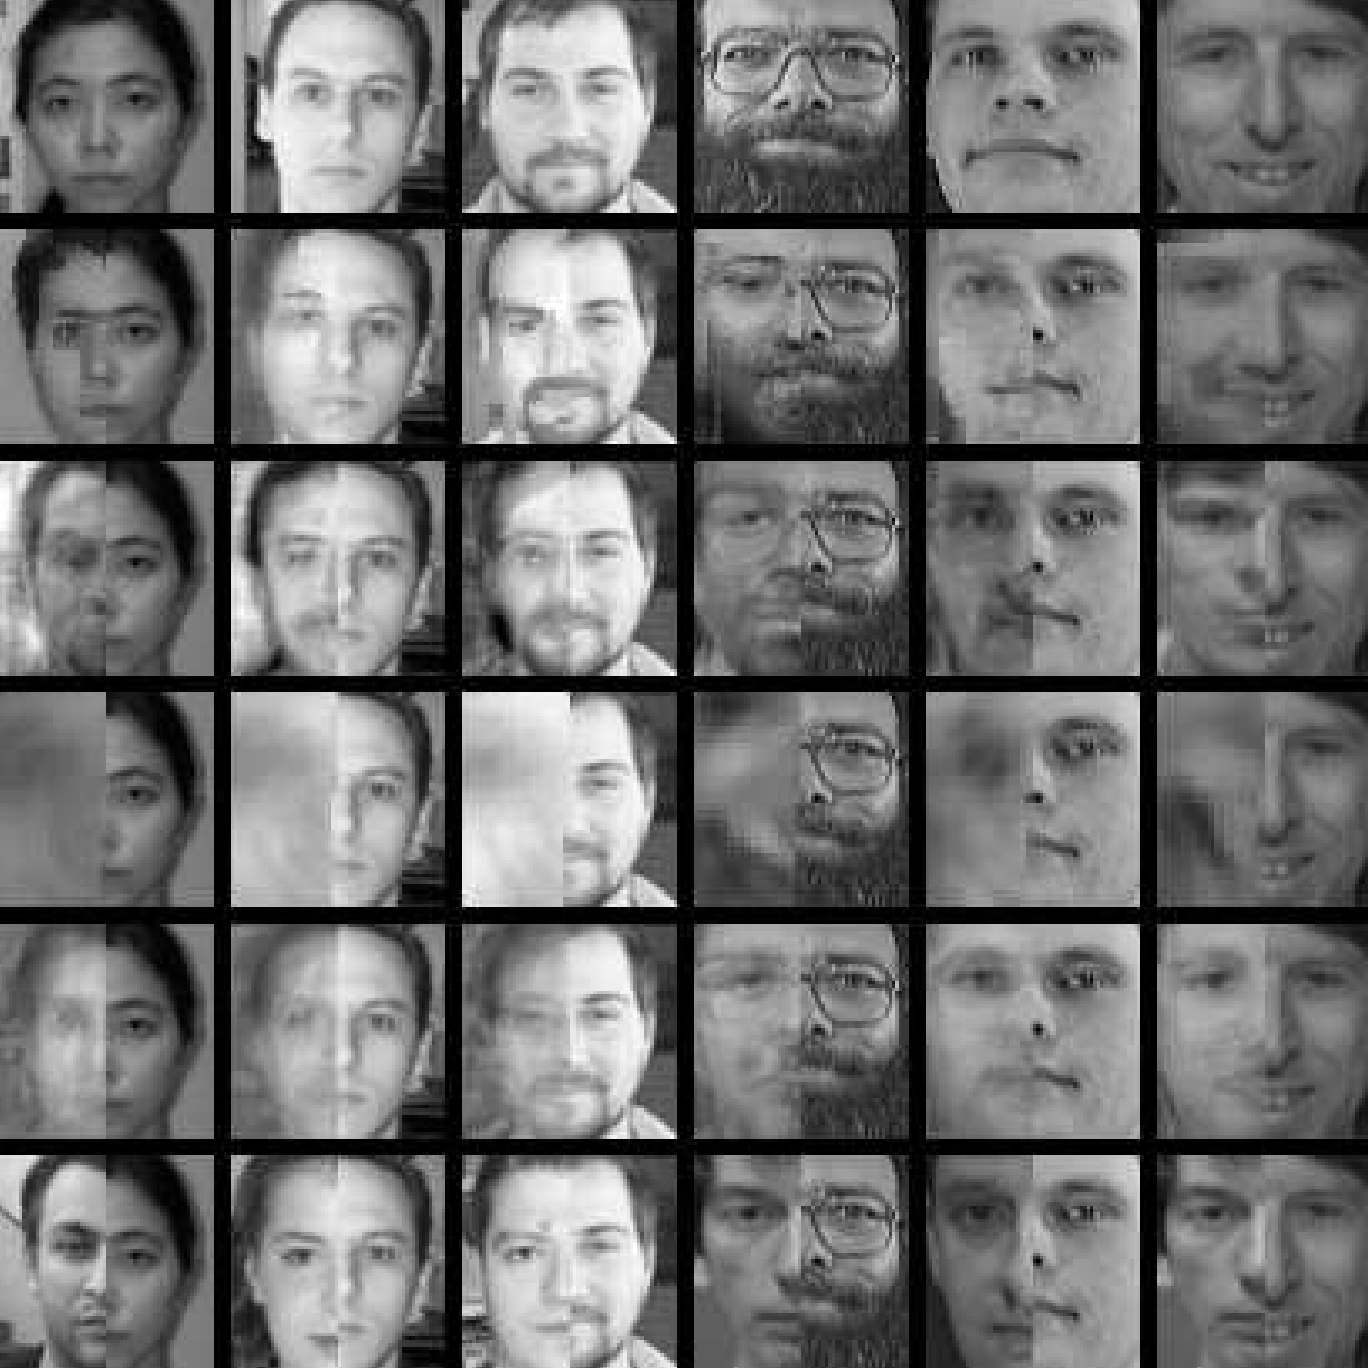
\includegraphics{figures/imagecompletion.png}
  }

  \caption[Sample face completions]{Sample face completions. Source: \citet{Poon2011}.}
  \label{fig:imagecompletion}
\end{figure}

Due to the $\mathcal{NP}$-Hardness of MAP inference in SPNs, various greedy approximation algorithms have been proposed, along with, more recently, some exact methods. However, these approaches have primarily focused on discrete SPNs, with only a few being extendable to continuous domains. Moreover, their experiments have not included continuous data. Finally, these methods typically search only for points corresponding to the modes of a specific component of the mixture, resulting in solutions of uncertain quality that are unable to guarantee even local optimality. Finding the modes of an SPN can help finding solutions to MAP inference.

Regarding cluster analysis, clustering can be approached by considering a density that represents the distribution of data in a given problem, and then taking its modes as representative of clusters. This approach has been successful in several applications; one example is image segmentation \citep{Cheng1995, Comaniciu2002, Li2007}.

We believe that finding modes of GSPNs can allow performing modal clustering with a class of densities that is more expressive and efficient than GMMs. Additionally, clustering is a valuable method for model analysis and model compression.

\section{Goal and methodology}
\label{sec:methodology}

Our goal is to develop a framework for locating modes of Gaussian Sum-Product Networks.

To achieve this, we will examine the connection between GSPNs and GMMs, survey literature concerning the modes of such models, and explore approaches for detecting them. We will propose an algorithm that adapts an EM-style fixed-point iteration method, known as Modal EM, to identify local maxima of GSPNs.

To validate our algorithm, we will carry out experiments on clustering.

\section{Contributions}
\label{sec:contributions}

The main contribution of this work is Modal EM for GSPNs, an algorithm designed to find modes of densities represented by Gaussian Sum-Product Networks. While this contribution has already been published during the author's postgraduate studies in proceedings of a conference \citep{Madeira2022}, this work offers a more comprehensive description of the algorithm and provides a formal proof of its correctness. In addition, we observe the relationship between Modal EM, a fixed-point iterative schema proposed by \citet{Carreira-Perpinan2000} and Mean-Shift. Furthermore, this thesis provides more context about the problem and reports additional experimental results. A paper about modal clustering with GSPNs containing some of the experiments of image segmentation reported in this document has been published in a workshop \citep{Madeira2023}.

\section{Organization}
\label{sec:organization}

The remaining chapters of this document are structured as follows.

Chapter \ref{cap:gmm} provides an overview of Gaussian Mixture Models and establishes the probability notations used throughout the thesis. We also review the literature related to the number of modes of GMMs and the techniques for mode-finding.

Chapter \ref{cap:spn} introduces Sum-Product Networks and explains how they are used for probabilistic reasoning. We discuss their relationship with mixture models, common methods to learning them from data, and the literature on Maximum-A-Posteriori (MAP) inference in discrete SPNs, which is closely related to finding the global maximum of the model.

Chapter \ref{cap:algorithm} details Modal EM for GSPNs, which is an adaptation of a method for locating maxima of GMMs to find modes of GSPNs. We describe the construction of the algorithm, prove its correctness and runtime complexity, and discuss some applications.

Chapter \ref{cap:experiments} presents experimental results obtained by using Modal EM for GSPNs in the aforementioned applications.

Finally, Chapter \ref{cap:final} concludes the work, provides some final thoughts and ideas for future research.


\chapter{Gaussian Mixture Models}
\label{cap:gmm}

In this chapter, we will review fundamental concepts of Gaussian Mixture Models (GMMs) and introduce some notations that will be used throughout this dissertation (Sections \ref{sec:gmm:fundamentals} and \ref{sec:gmm:models}). We will then discuss the literature on the number of modes (local maxima) in GMMs (Section \ref{sec:gmm:nmodes}) and, finally, approaches to find such modes (Section \ref{sec:gmm:fmodes}).

We assume some basic knowledge of probabily theory; gentle introductions are found in the works of \citet{Jaynes2003} and \citet{Kadane2011}.

\section{Gaussian distribution}
\label{sec:gmm:fundamentals}

We will use uppercase letters to denote random variables (RVs) and lowercase letters to denote assignments of RVs.

\begin{definition}[Univariate Gaussian]
  An RV $X$ has a \textbf{univariate Gaussian distribution} with mean $\mu$ and variance $\sigma^2$, denoted $X \sim \mathcal{N}\left(\mu, \sigma^2\right)$, if it has the probability density function

  \begin{equation}
    p(x) = \frac{1}{\sqrt{2\pi} \sigma} e^{-\frac{(x - \mu)^2}{2\sigma^2}} \, .
  \end{equation}
\end{definition}

\noindent We will use $p( \cdot )$ to denote probability density functions (PDFs). Figure \ref{fig:gaussian}(a) shows the PDFs of three univariate Gaussian distributions.

\begin{figure}
  \begin{minipage}{0.5\textwidth}
    \centering
    \scalebox{0.8}{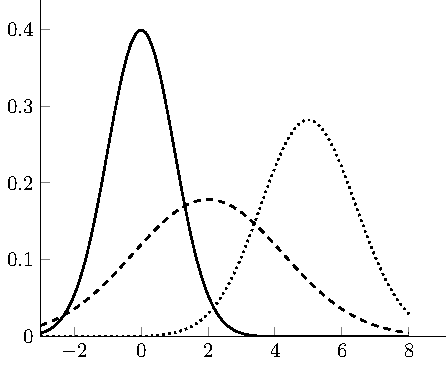
\includegraphics{figures/gaussian-a.pdf}}

    (a)
  \end{minipage}\begin{minipage}{0.5\textwidth}
    \centering
    \scalebox{0.8}{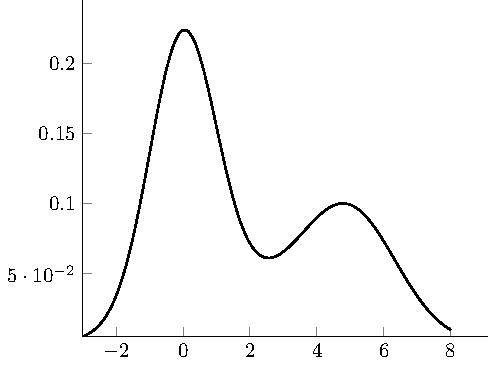
\includegraphics{figures/gaussian-b.pdf}}

    (b)
  \end{minipage}

  \caption[Plot of Gaussian distributions and GMM]{
    \textbf{(a)} Plot of the PDFs of three Gaussian distributions: $\mathcal{N}(0, 1)$ (solid line), $\mathcal{N}(2, 5)$ (dashed line) and $\mathcal{N}(5, 2)$ (dotted line).
    \textbf{(b)} Plot of the PDF of a univariate Gaussian mixture model, $X \sim 0.5 \mathcal{N}(0, 1) + 0.2 \mathcal{N}(2, 5) + 0.3 \mathcal{N}(5, 2)$.
  }
  \label{fig:gaussian}
\end{figure}

Gaussian distributions are extended to the multivariate case:

\begin{definition}[Multivariate Gaussian]
  A random vector $\mathbf{X} = (X_1, \cdots, X_n)$ is said to have a \textbf{multivariate Gaussian distribution} with mean $\boldsymbol{\mu}$ (a $n$-dimensional vector) and covariance matrix $\boldsymbol{\Sigma}$ (to not be confused with summation sign), $\mathbf{X} \sim \mathcal{N}\left(\boldsymbol{\mu}, \boldsymbol{\Sigma}\right)$, if:

  \begin{equation}
    p(\mathbf{x}) = 2\pi^{-\frac{n}{2}} \textrm{det}\left(\boldsymbol{\Sigma}\right)^{\frac{1}{2}} e^{-\frac{1}{2}\left(\mathbf{x}-\boldsymbol{\mu}\right)^T\boldsymbol{\Sigma}^{-1}\left(\mathbf{x}-\boldsymbol{\mu}\right)} \, .
  \end{equation}
\end{definition}

\noindent We will denote random vectors using bold uppercase letters and assignments of random vectors using bold lowercase letters. Random vectors and sets of random variables will be used interchangeably for the sake of simplicity in notation.

$\boldsymbol{\Sigma}$ is a symmetric $n \times n$ matrix and the value $\Sigma_{i,j}$ is, by definition, the covariance between variables $X_i$ and $X_j$, $\operatorname{Cov}[X_i, X_j]$:

\begin{equation}
  \Sigma_{i,j} := \operatorname{Cov}[X_i, X_j] = \operatorname{E}\left[(X_i - \mu_i)( X_j - \mu_j)\right] \, .
\end{equation}

In general, RVs may be uncorrelated but statistically dependent. In the case of multivariate Gaussian distributions, two or more variables are uncorrelated if and only if they are independent. The product of PDFs of independent Gaussian RVs is a multivariate Gaussian distribution with a diagonal covariance matrix.

A Gaussian distribution is said to be \textbf{isotropic} (or \emph{spherical}) if its covariance matrix is diagonal and all variables have the same variance. Formally, a distribution in $\mathbb{R}^d$ is isotropic if $\mathbf{\Sigma} = \sigma^2\mathbf{I}_d$ for some $\sigma \in \mathbb{R}$, where $\mathbf{I}_d$ is the identity matrix of size $d$.

\section{Mixture models}
\label{sec:gmm:models}

A finite \textbf{mixture model} is a distribution formed by a convex combination of distributions. Formally, if $p_1(\mathbf{X}), \cdots, p_n(\mathbf{X})$ are densities over a random vector $\mathbf{X}$, we can define a finite mixture model $p(\mathbf{X})$ of components $p_1, \cdots, p_n$ by choosing weights $w_1, \cdots, w_n \geq 0$ such that $\sum_{z=1}^n w_z = 1$ and making:

\begin{equation}
  p(\mathbf{x}) = \sum_{z=1}^n w_z p_z(\mathbf{x}) \, .
\end{equation}

We can interpret the mixture coefficients $w_z$ as a categorical \textbf{latent variable} (usually denoted $Z$) such that $p(z) = w_z$, $p(\mathbf{x} \mid z) = p_z(\mathbf{x})$, and

\begin{equation}
  p(z, \mathbf{x}) = p(z) p(\mathbf{x} \mid z) \, .
\end{equation}

\noindent Variables in $\mathbf{X}$ are called \textbf{observable variables} in contrast to latent variables. Then, computing $p(\mathbf{x})$ consists in marginalizing the variable $z$:

\begin{eqnarray}
  p(\mathbf{x}) & = & \sum_{z=1}^n p(z) p(\mathbf{x}, z) \\
  & = & \sum_{z=1}^n w_z p_z(\mathbf{x}) \, .
\end{eqnarray}

\begin{definition}[Gaussian Mixture]
  A \textbf{Gaussian Mixture Model} (GMM) is a mixture model of Gaussian distributions.
\end{definition}

\noindent Figure \ref{fig:gaussian}(b) depicts a univariate GMM, but in this work, we will mainly deal with multivariate GMMs.

A GMM is said to be \textbf{homoscedastic} if it has equal covariance matrices for all its components, and is said to be \textbf{isotropic} if its components are isotropic.

\section{Number of modes}
\label{sec:gmm:nmodes}

The \textbf{modes}, or local maxima, of a density in $d$ dimensions are the points of the PDF at which it achieves a local maximum value.

\begin{definition}[Mode]
  A point $\mathbf{x}^\star \in \mathbb{R}^d$ is a mode of $f(\mathbf{x})$ if there exists a neighborhood\footnote{Given a $\delta > 0$, a \emph{neighborhood} of $\mathbf{x}^\star$ is the set of points $\mathbf{x} \in \mathbb{R}^d$ which satisfy $||\mathbf{x}^\star - \mathbf{x}||_2 < \delta$.} of $\mathbf{x}^\star$ such that $f(\mathbf{x}^\star) \geq f(\mathbf{x})$ for all $\mathbf{x}$ within that neighborhood.
\end{definition}

While a probability distribution can have multiple modes (for example, uniform distributions have infinitely many modes), a Gaussian distribution has only one mode, namely, its mean. At first glance, one might assume that the number of modes of a GMM would be small and easy to determine, since it is a combination of a finite number of Gaussian components. However, the number of modes that a mixture of $k$ Gaussians in $\mathbb{R}^d$ can possess is surprisingly unknown, not proven to be finite, and identifying such modes remains a challenging problem.

Let $m(d, k)$ denote the maximal number of modes for $d$-dimensional Gaussian mixtures with $k$ components. As previously stated, $m(d, 1) = 1$, because a GMM with one component is simply a Gaussian distribution. Numerous studies have examined the lower and upper bounds of $m(d, k)$ for greater values of $d$ and $k$, and we will briefly review some of the most recent ones, such as the ones by \citet{Carreira-Perpinan2003a}, \citet{Ray2012}, and \citet{Amendola2019}.

While \citet{Carreira-Perpinan2003} proved that the number of modes of univariate GMMs is limited by its number of components ($m(1, k) = k$), the result does not hold in higher dimensions. Figure \ref{fig:amendola}(a) presents a counterexample that shows the mixture of two Gaussians in two dimensions, $\mathbf{X}_1 \sim \mathcal{N}\left(\boldsymbol{\mu}_1, \boldsymbol{\Sigma}_1\right)$ and $\mathbf{X}_2 \sim \mathcal{N}\left(\boldsymbol{\mu}_2, \boldsymbol{\Sigma}_2\right)$, where $\boldsymbol{\mu}_1 = (1, 0)$, $\boldsymbol{\Sigma}_1 = [(1, 0), (0, 0.1)]$, $\boldsymbol{\mu}_2 = (0, 1)$, and $\boldsymbol{\Sigma}_2 = [(0.1, 0), (0, 1)]$, with coefficients $w_1 = w_2 = \frac{1}{2}$. The mixture has two modes near the original means at $(1, 0)$ and $(0, 1)$, and a third mode near the origin.

\begin{figure}
  \begin{minipage}{0.3333\textwidth}
    \centering
    \scalebox{0.085}{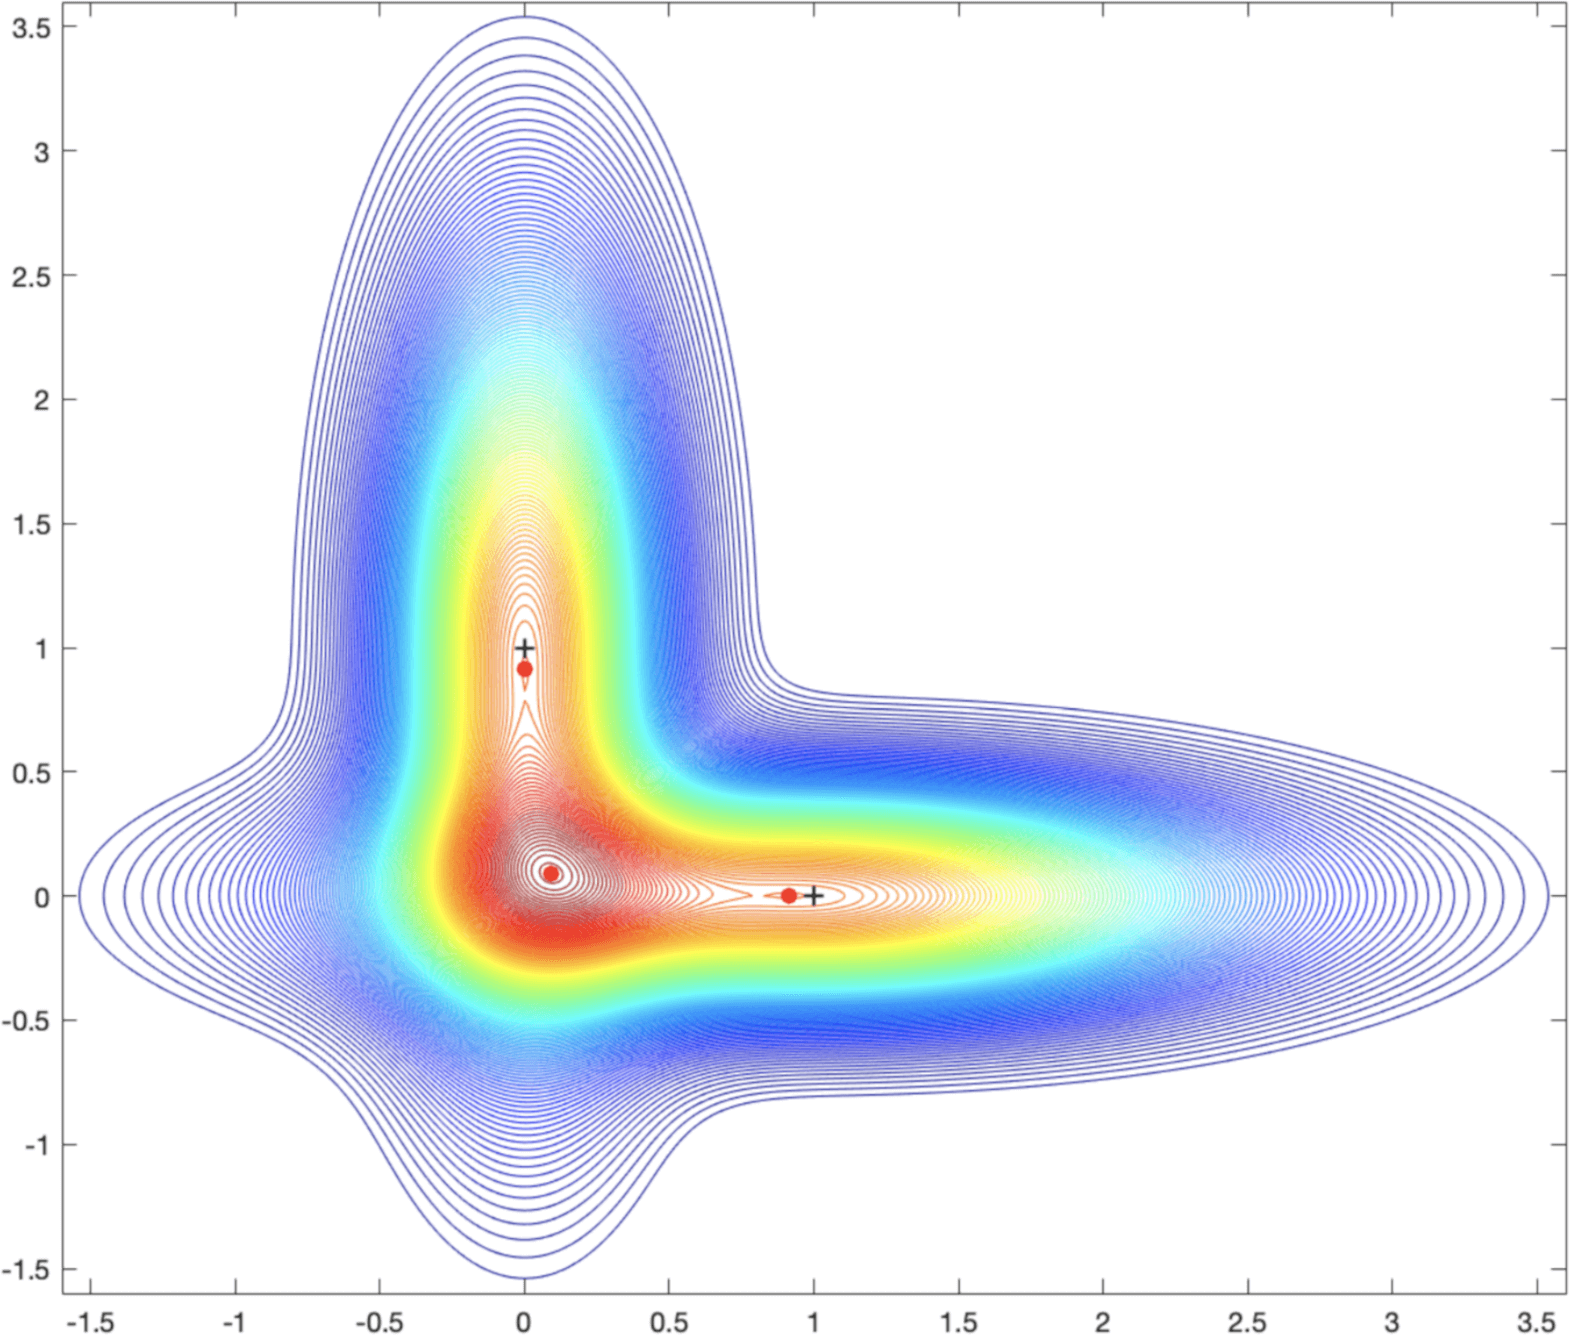
\includegraphics{figures/amendola1.png}}

    (a)
  \end{minipage}\begin{minipage}{0.3333\textwidth}
    \centering
    \scalebox{0.085}{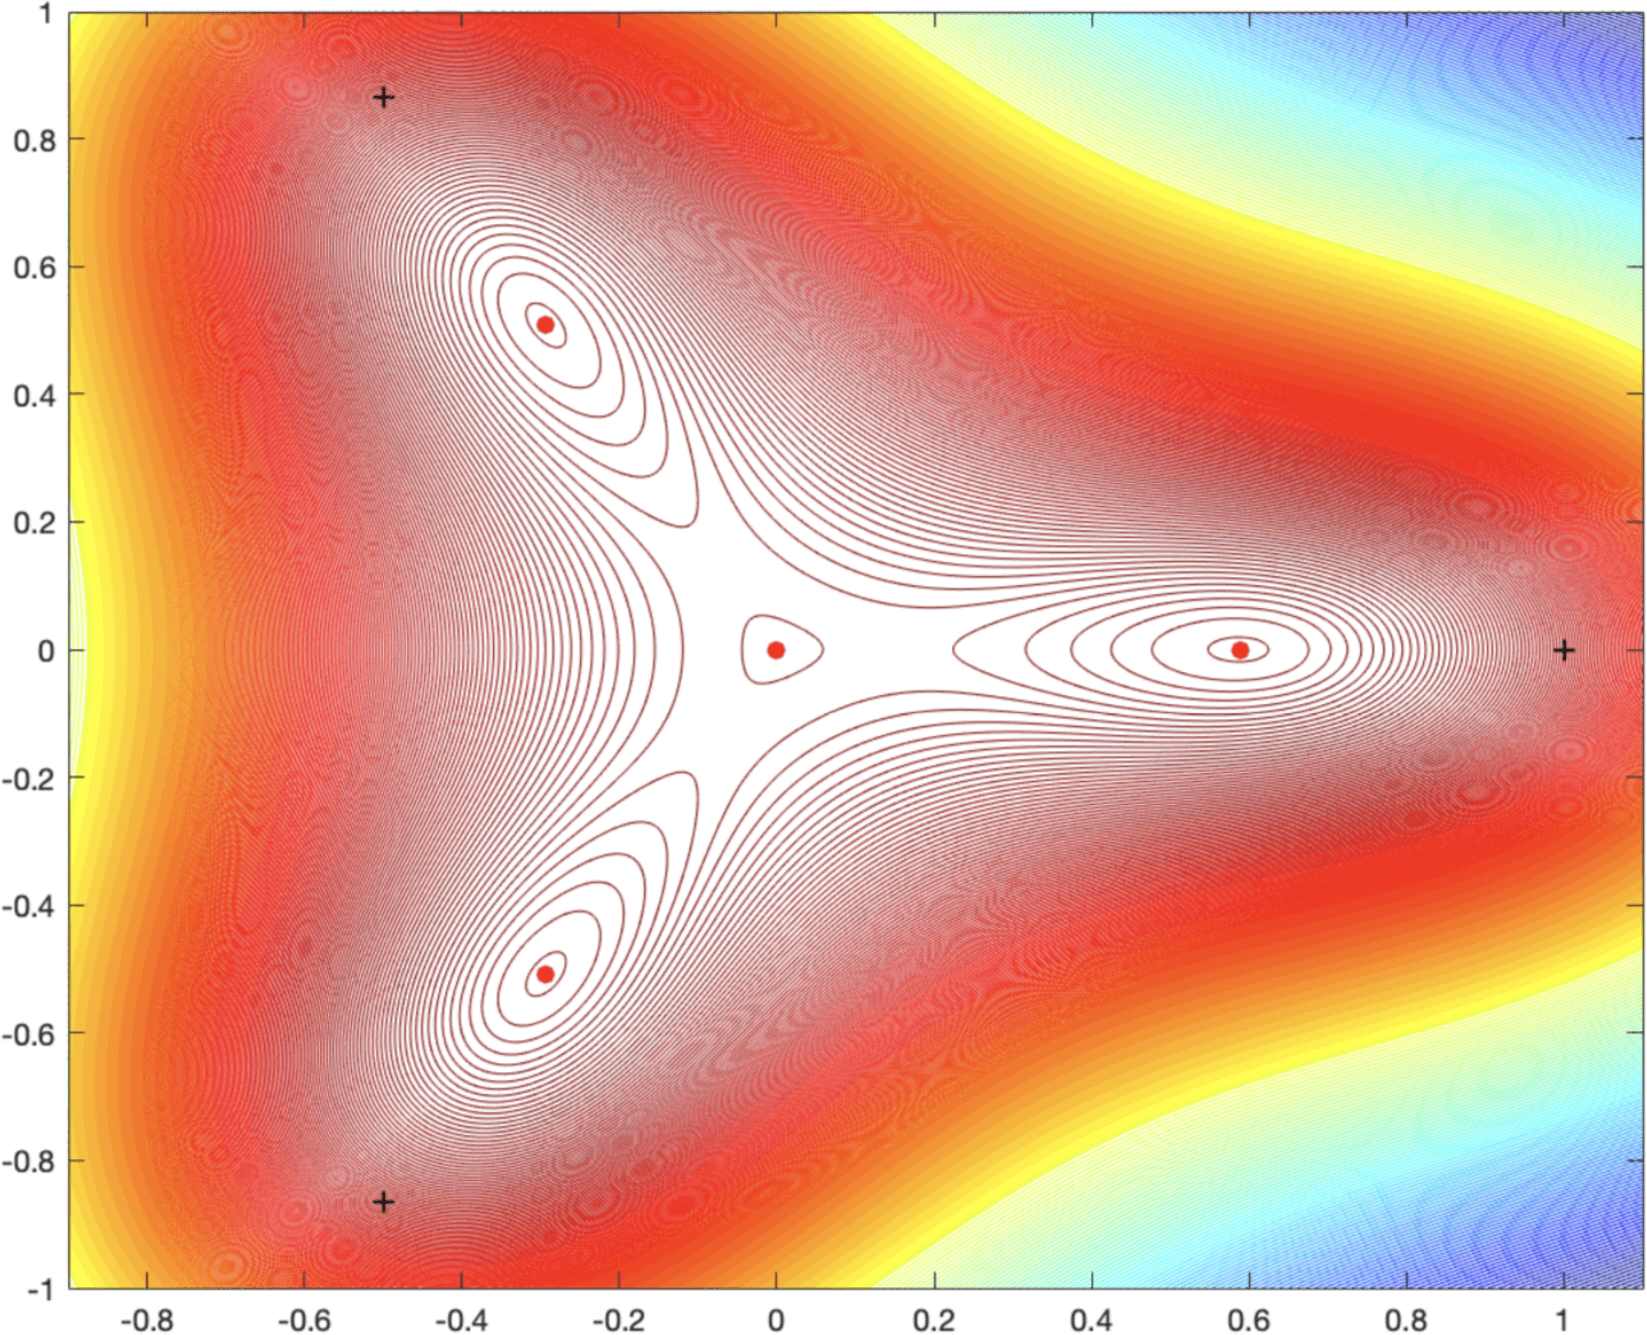
\includegraphics{figures/amendola2.png}}

    (b)
  \end{minipage}\begin{minipage}{0.3333\textwidth}
    \centering
    \scalebox{0.085}{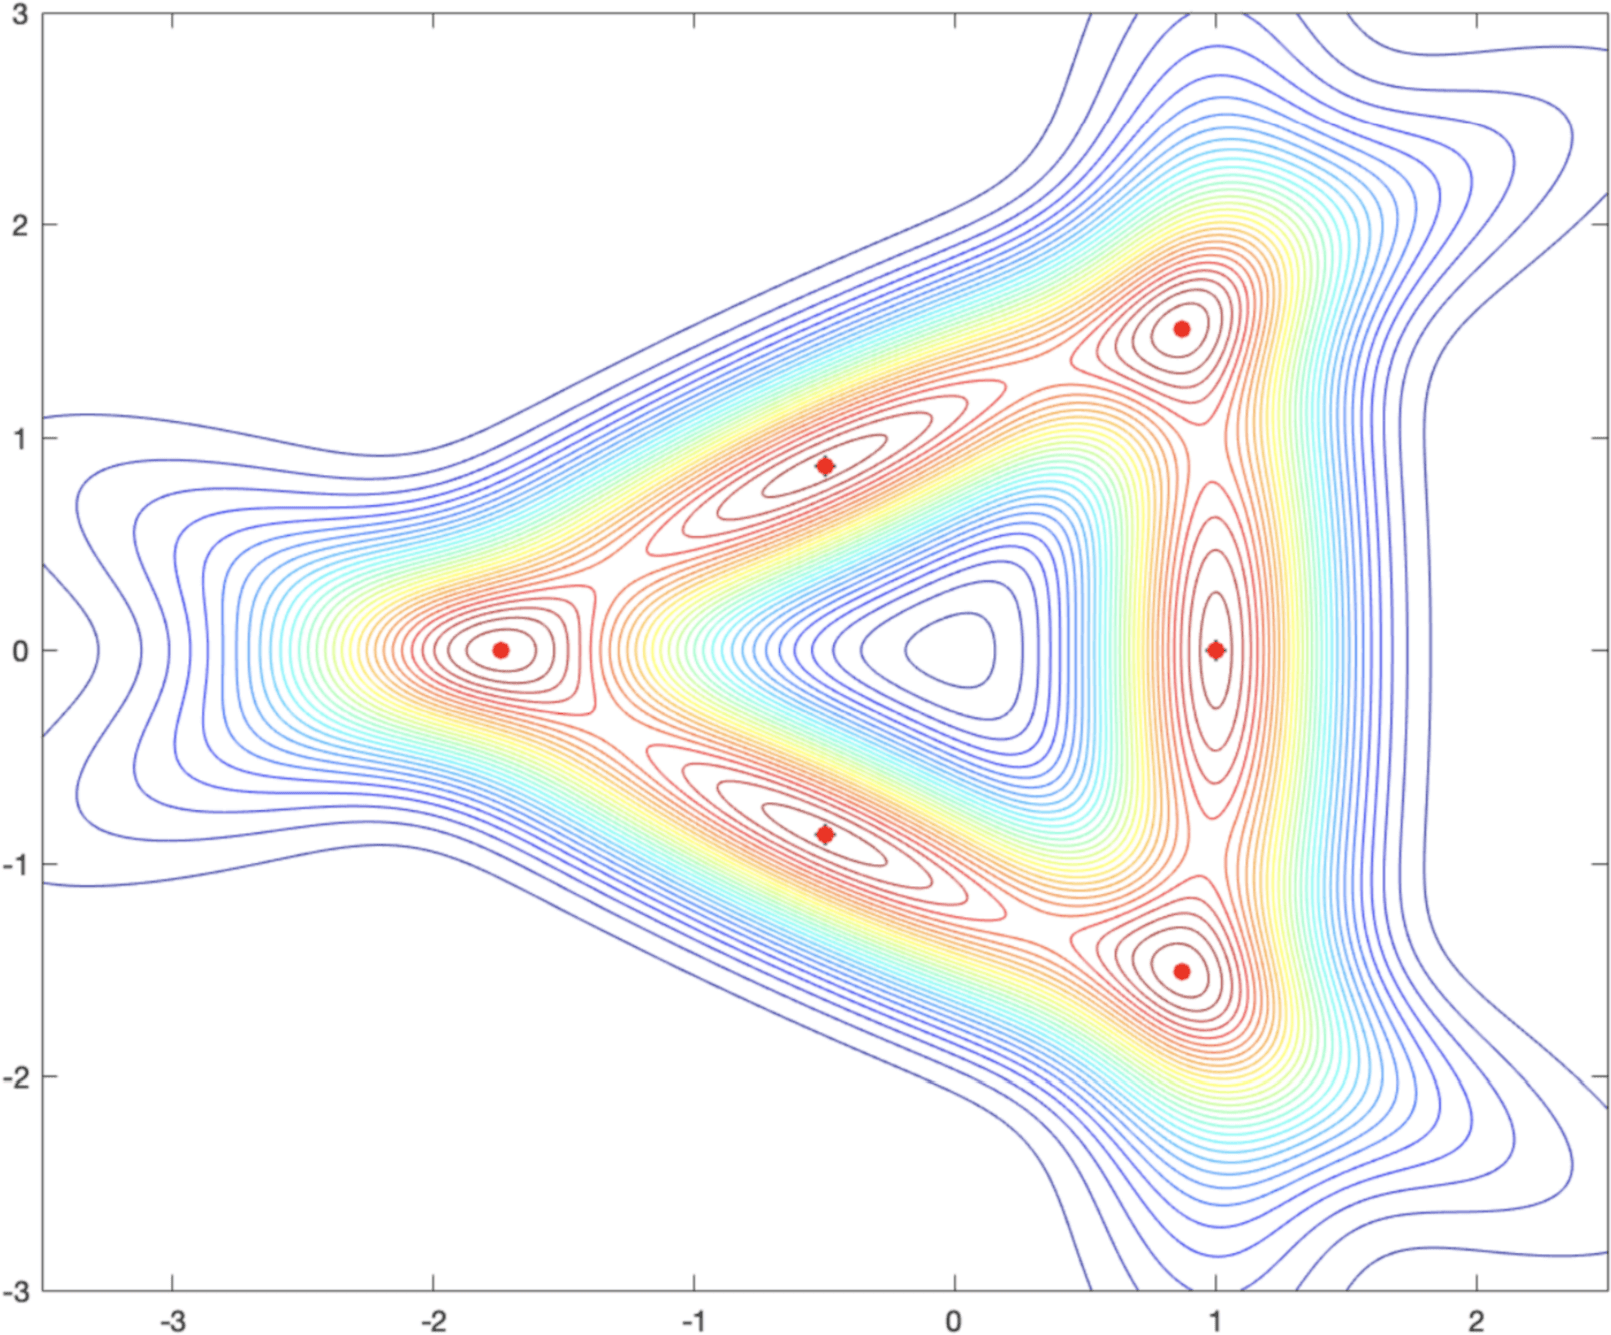
\includegraphics{figures/amendola3.png}}

    (c)
  \end{minipage}

  \caption[Bivariate GMMs with more modes than components]{
    Bivariate GMMs with more modes than components. Component means are represented by $+$ (black crosses) and GMM modes are represented by {\color{red} $\bullet$} (red bullets).
    \textbf{(a)} 2 components and 3 modes.
    \textbf{(b)} 3 isotropic components and 4 modes.
    \textbf{(c)} 3 components and 6 modes.
    Source: \citet{Amendola2019}.
  }
  \label{fig:amendola}
\end{figure}

In a conjecture, the same article suggested that the number of modes of an isotropic GMM could not exceed its number of components. However, a counterexample presented by J. J. Duistermaat \citep{Carreira-Perpinan2003a} proved that conjecture to be false. The counterexample, shown in Figure \ref{fig:amendola}(b), consists of an homoscedastic isotropic GMM with three components positioned at the vertices of an equilateral triangle and four modes. The mixture is formed by $\mathbf{X}_1 \sim \mathcal{N}\left((1, 0), \sigma^2I_2\right)$, $\mathbf{X}_2 \sim \mathcal{N}\left(\left(-\frac{1}{2}, \frac{\sqrt{3}}{2}\right), \sigma^2I_2\right)$, and $\mathbf{X}_3 \sim \mathcal{N}\left(\left(-\frac{1}{2}, -\frac{\sqrt{3}}{2}\right), \sigma^2\mathbf{I}_2\right)$, where $\sigma^2 = 0.53$, $\mathbf{I}_2$ is the identity matrix of size $2 \times 2$, and $w_1 = w_2 = w_3 = \frac{1}{3}$.

\citet{Ray2012} proved that one can get as many as $d+1$ modes from a Gaussian mixture of two components in $\mathbb{R}^d$ and that is always possible to find a GMM of only two components with $d+1$ modes in $d$ dimensions, therefore $m(d, 2) = d+1$. GMMs with more components can get much more complex. To give an example, Figure \ref{fig:amendola}(c) shows a GMM in $\mathbb{R}^2$ with 3 components and 6 modes, demonstrating that $m(2, 3) \geq 6$.

To date, the most stringent lower and upper bounds for $m(d, k)$ were established by \citet{Amendola2019}. They demonstrate that, given integers $k, d \geq 2$, there exists a mixture of $k$ Gaussians in $d$ dimensions with at least ${k \choose d} + k$ modes, i.e., $m(d, k) \geq {k \choose d} + k$. Additionally, they prove that the number of non-degenerate stationary points for a GMM with $k$ components in $d$ dimensions is bounded by $2^{d+{k \choose 2}}(5+3d)^k$. That means that, assuming that every mixture of $k$ Gaussians in $\mathbb{R}^d$ has finitely many modes, then

\begin{equation}
  {k \choose d} + k \, \leq \, m(d, k) \, \leq \, 2^{d+{k \choose 2}}\left(5+3d\right)^k.
\end{equation}

That result shows that the lower bound for the number of modes in a GMM is unexpectedly large, especially for mixtures with many components. For instance, this bound implies that there exists a GMM with 100 components in $\mathbb{R}^{50}$ with more than $10^{29}$ modes, a fact that seems counterintuitive.

It is also surprising that there is still no conclusive evidence as to whether the number of modes of a GMM is always finite. Although it may seem intuitive that a finite mixture of Gaussians would not contain non-degenerate critical points, the lack of proof leaves the possibility that there may not exist a finite upper bound for $m(k, d)$.

Nevertheless, it is important to note that in real-life scenarios, the number of modes of GMMs does not seem to explode, at least when the components are isotropic. According to \citet{Carreira-Perpinan2003a}, it is very rare to find GMMs with more modes than components in such cases.

\section{Finding modes of GMMs}
\label{sec:gmm:fmodes}

The results regarding the number of modes of GMMs provide insight into the intricate nature of the modes landscape. In this study, we investigate how to find modes of GMMs, and two fundamental initial questions are: (1) where are the modes located, and (2) which specific modes we aim to find.

On the question of \emph{where are the modes located}, for isotropic GMMs it is proven that the modes lie inside the convex hull of the component centroids \citep{Amendola2019}. However, this property does not hold for non-isotropic GMMs, as illustrated by a counter-example in $\mathbb{R}^2$ shown in \ref{fig:amendola}(a).

As an exercise of imagination, we propose the conjecture that, in general, the modes of a GMM reside within the hyperrectangle formed by the minimum and maximum values of each coordinate in the component centroids. Even if that is not always true, we can argue that such modes have greater practical relevance: the primary applications of finding modes of GMMs are either finding probable values of a model or, notably, clustering in domains such as data analysis, pattern recognition and image processing. In this context, a mode is considered a representative of a cluster, and a mode located outside the space between the centroids may not be a suitable representative for a cluster.

As for \emph{which specific modes we aim to find}, it is usually not crucial to identify all the modes of a model, but rather the most probable one or modes to which data points converge. That led us to investigate two problems: finding global maxima and finding modes starting from points.

\vspace{1em}

Starting with global maxima, seeking such mode has applications such as real-time object tracking in computer vision \citep{Shen2005} and has been investigated by \citet{Pulkkinen2014} in his PhD thesis.

\citet{Pulkkinen2013} introduced a method for smoothing a given GMM using Gaussian convolution. This technique effectively eliminates undesired local maxima while preserving the fundamental structure of the GMM. The convolved Gaussian mixture has been shown to be strictly concave under mild assumptions, and therefore has a unique maximum. Notably, their proposed method operates globally, meaning it is not dependent on the starting point, and has the ability to identify a significant mode, although not necessarily the maximum one. In the same paper, the authors argued that finding the global mode of a Gaussian kernel density estimate, which is a special case of a Gaussian mixture, is a difficult global optimization problem.

\vspace{1em}

Finding multiple modes starting from points is usually done using hill-climbing methods, which are designed to iteratively ascend from any initial point. We will briefly review Gradient Ascent, Mean-Shift and Modal EM.

\subsubsection{Gradient ascent}

For differentiable functions, \textbf{Gradient Ascent} \citep{Murphy2012} is a popular iterative optimization algorithm to find a mode. At each step, the algorithm computes the gradient of the function at the current point ($\mathbf{x}^{(r)}$) and updates the point in the direction of the gradient: $\mathbf{x}^{(r+1)} \gets \mathbf{x}^{(r)} + \gamma \nabla f\left(\mathbf{x}^{(r)}\right)$. However, a major issue with this method is that it heavily relies on the choice of a step size parameter, $\gamma \in \mathbb{R}+$, which must be carefully selected to ensure that $f\left(\mathbf{x}^{(r+1)}\right) \geq f\left(\mathbf{x}^{(r)}\right)$ for all $r$. Finding an appropriate step size can be a difficult and costly process, as it often requires multiple iterations of its own. This can make Gradient Ascent slow to converge.

\subsubsection{Mean-Shift}

In the field of cluster analysis, a common technique to locate the modes of a density is \textbf{Mean-Shift} and its variants \citep{Fukunaga1975, Carreira-Perpinan2015}. Traditionally, the Mean-Shift algorithm does not take a model (density function) as input. Instead, it works directly with data points by defining a kernel density estimate, making it suitable for clustering since the input is similar to that of other clustering algorithms such as $k$-means (except for not requiring a $k$ parameter). The algorithm iteratively shifts a point to the average of data points in its neighborhood until the point does not change.

Formally, let data be a finite set $\mathbf{S} = \left\{\mathbf{s}_n\right\}_{n=1}^N \subset \mathbb{R}^d$, so that a $\mathbf{s} \in \mathbf{S}$ corresponds to a single data point in $\mathbb{R}^d$. Let $\mathbf{x}^{(0)}$ be a point in $\mathbb{R}^d$. The \textbf{sample mean} at $\mathbf{x}$ is defined as:

\begin{equation}
  m\left(\mathbf{x}\right) := \frac{
    \sum_{\mathbf{s} \in \mathbf{S}} K\left(\mathbf{s}-\mathbf{x}\right) \mathbf{s}
  }{
    \sum_{\mathbf{s} \in \mathbf{S}} K\left(\mathbf{s}-\mathbf{x}\right)
  } \, ,
\end{equation}

\noindent where $K(\mathbf{x})$ is a \emph{kernel} function that comprises a bandwidth parameter $\lambda$. Commonly, flat kernels and Gaussian kernels have been used. A \textbf{flat kernel} is the characteristic function $F$ of the $\lambda$-ball in $\mathbb{R}^d$:

\begin{equation}
  F(\mathbf{x}) := \begin{cases}
    1 & \text{ if } ||\mathbf{x}|| \leq \lambda \, , \\
    0 & \text{ if } ||\mathbf{x}|| > \lambda \, ,
  \end{cases}
\end{equation}

\noindent and a \textbf{Gaussian kernel} is defined as:

\begin{equation}
  G(\mathbf{x}) := e^{-\frac{||\mathbf{x}||^2}{2\lambda^2}} \, .
\end{equation}

\noindent (In this case the parameter $\lambda$ is the standard deviation of the Gaussian function, normally denoted as $\sigma$).

The difference $m(\mathbf{x}) - \mathbf{x}$ is called \textbf{mean shift vector} and, at each step, the Mean-Shift algorithm updates the point in its direction, making $\mathbf{x}^{(r+1)} \leftarrow m\left(\mathbf{x}^{(r)}\right)$.

Mean-Shift has been re-discovered, adapted and modified for various density functions in several studies \citep{Cheng1995, Carreira-Perpinan2000, Comaniciu2002}. The algorithm was extended to use mixture components instead of kernel density estimation from data points. In the case of Gaussian Mixture Models, it has been demonstrated that the Mean-Shift algorithm is equivalent to a Expectation-Maximization method named Modal EM \citep{Carreira-Perpinan2007, Chacon2019}, which we will describe next.

\subsubsection{Modal EM}

\citet{Carreira-Perpinan2000} proposed another fixed-point iterative schema as follows. Given a GMM $p(\mathbf{x}) = \sum_{z=1}^n w_z p_z(\mathbf{x})$ and a point $\mathbf{x}^{(r)}$,

\begin{equation}
  \label{eq:mem:gmm}
  \mathbf{x}^{(r+1)} \gets \frac{
  \sum_{z=1}^n w_z p_z\left(\mathbf{x}^{(r)}\right) \boldsymbol{\Sigma}_z^{-1} \boldsymbol{\mu}_z
  }{
  \sum_{z=1}^n w_z p_z\left(\mathbf{x}^{(r)}\right) \boldsymbol{\Sigma}_z^{-1}
  } \, .
\end{equation}

\noindent This algorithm has some advantages over Gradient Ascent, such as not requiring any additional parameters. Additionally, it was shown to be a Expectation-Maximization (EM) method, which facilitates its convergence analysis. As such, it approaches a mode from almost any initial point and monotonically increases the density value or leaves it unchanged: $p(\mathbf{x}^{(r+1)}) \geq p(\mathbf{x}^{(r)})$, and $\mathbf{x}^{(r+1)} \neq \mathbf{x}^{(r)} \Rightarrow p(\mathbf{x}^{(r+1)}) > p(\mathbf{x}^{(r)})$.

Independently, \citet{Li2007} introduced an EM-style method named \textbf{Modal EM} which is equivalent to the schema proposed by \citet{Carreira-Perpinan2000} for GMMs, as we will observe in Chapter \ref{cap:algorithm}. To apply Modal EM, one starts with a mixture density of $\tau$ components, $p(\mathbf{x}) = \sum_k^\tau w_k p^k(\mathbf{x})$, and an initial point $\mathbf{x}^{(0)}$. The method then alternates between the following two steps, starting with $r = 0$:

\begin{equation}
  \label{eq:mem:expectation}
  \text{\textbf{Expectation}: Let }
  q_k = \frac{w_k p^k\left(\mathbf{x}^{(r)}\right)}{p\left(\mathbf{x}^{(r)}\right)},
  \text{ for } k = 1, \cdots, \tau \, .
\end{equation}

\begin{equation}
  \label{eq:mem:maximization}
  \text{\textbf{Maximization}: Compute }
  \mathbf{x}^{(r+1)} = \arg\max_\mathbf{x} \sum_k^\tau q_k \log p^k\left(\mathbf{x}\right) \, .
\end{equation}


\chapter{Sum-Product Networks}
\label{cap:spn}

In this chapter, we review some literature about SPNs. We will begin by introducing the definition and fundamental concepts of SPNs (Section \ref{sec:spn:fundamentals}) and showing how an SPN is evaluated (Section \ref{sec:spn:evaluation}). Then, we will leverage the relation between SPNs and mixture models, and, particularly, the relation between GSPNs and GMMs (Section \ref{sec:spn:trees}). Next, we will show how SPNs are learned from data (Section \ref{sec:spn:learning}). Finally, we will review the literature on performing Maximum-A-Posteriori inference in SPNs, which is equivalent to finding a global maximum (Section \ref{sec:spn:map}).

Assuming the reader's familiarity with standard definitions of graph theory \citep{Bondy2008}, we proceed to use them throughout this work without further elaboration.

\section{Fundamentals}
\label{sec:spn:fundamentals}

We define the \textbf{scope} of a Sum-Product Network as the set of variables that appear in it, and we define \textbf{Sum-Product Network} (SPN) recursively \citep{Gens2013}.

\begin{definition}[Sum-Product Network]
  A Sum-Product Network is defined as follows:

  \begin{itemize}
    \item Any tractable univariate distribution is an SPN.
    \item Any product of SPNs with disjoint scopes is an SPN.
    \item Any weighted sum of SPNs with the same scope and nonnegative weights adding up to $1$ is an SPN.
    \item Nothing else is an SPN.
  \end{itemize}
\end{definition}

SPNs are commonly represented as rooted directed acyclic graphs with three types of nodes:

\begin{itemize}
  \item A univariate distribution is represented as a leaf.
  \item A product of SPNs is represented as an internal product node (denoted by $\times$) with nonweighted edges to the SPNs which it multiplies.
  \item A weighted sum of SPNs is represented as an internal sum node (denoted by $+$) with weighted edges to the SPNs which it sums.
\end{itemize}

The recursive construction of an SPN, as defined above, ensures that every node in the network readily represents a probability distribution over its scope. Specifically, leaves are distributions by definition, product nodes represent distributions under the assumption of independence among their children distributions, and sum nodes represent mixture distributions \citep{Peharz2015}.

\begin{figure}
  \begin{minipage}{0.5\textwidth}
    \centering
    \scalebox{1}{
      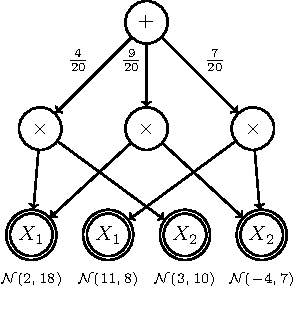
\includegraphics{figures/gspn-b.pdf}
    }

    (a)
  \end{minipage}\begin{minipage}{0.5\textwidth}
    \centering
    \scalebox{0.82}{
      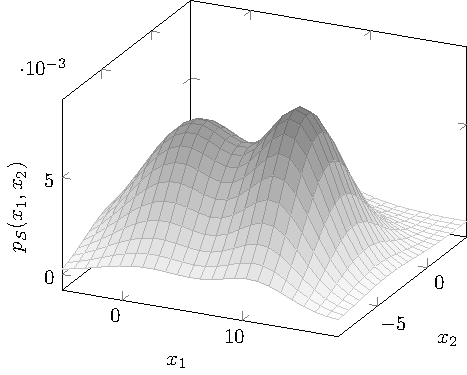
\includegraphics{figures/gspn-c.pdf}
    }

    (b)
  \end{minipage}

  \caption[A GSPN and a plot of its PDF]{
    \textbf{(a)} A SPN $\mathcal{S}$ with Gaussian leaves.
    \textbf{(b)} Plot of the PDF of the distribution $\mathcal{S}$.
  }
  \label{fig:gspn}
\end{figure}

SPNs can be constructed using discrete, continuous, or hybrid (mixed) variables. Although many studies have been conducted on SPNs based on categorical random variables, there are many real-world applications that are better suited to continuous variables \citep{Jaini2016}. In this study, we concentrate on SPNs that use continuous RVs (learned from continuous data), particularly SPNs with univariate Gaussian distributions at their leaves. We refer to these networks as \textbf{Gaussian Sum-Product Networks} (GSPNs).

\begin{definition}[Gaussian Sum-Product Network]
  A Gaussian Sum-Product Network is a Sum-Product Network with only univariate Gaussian distributions at their leaves.
\end{definition}

\noindent Figure \ref{fig:gspn}(a) displays an example of a GSPN, and \ref{fig:gspn}(b) depicts its probability density function. Although marginal inference works the same way for discrete and continuous SPNs (except that discrete SPNs compute probability masses, whereas continuous SPNs compute densities), certain algorithms that operate on discrete SPNs may not function with continuous SPNs and vice versa.

\section{Inference in SPNs}
\label{sec:spn:evaluation}

The process of performing reasoning in probabilistic models is called \textbf{inference}. SPNs allow performing marginal inference and conditional inference in linear time in the size of the network.

Given an SPN $\mathcal{S}$, we denote its probability distribution function as $\mathcal{S}(\cdot)$. To perform marginal inference, that is, to compute the probability of a valuation $\mathbf{x}$ of RVs $\mathbf{X}$ in the SPN $\mathcal{S}$, $\mathcal{S}(\mathbf{X} = \mathbf{x})$, we traverse the graph in reverse topological order. For a node $u$ in an SPN $\mathcal{S}$, let $u(\mathbf{x})$ denote the value of the node $u$ in the SPN given the valuation $\mathbf{X} = \mathbf{x}$ restricted to the RVs in the scope of $u$ and let $\ch(u)$ denote the children of $u$ in the DAG. Then,

\begin{enumerate}
  \item If $u$ is a leaf, $u(x)$ is the density of $x$ of its corresponding univariate distribution over $X$.
  \item If $u$ is a product node, $u(\mathbf{x})$ is the product of its children:

        \begin{equation}
          u(\mathbf{x}) = \prod_{v \in \ch(u)} v(\mathbf{x}) \, .
        \end{equation}
  \item If $u$ is a sum node, $u(\mathbf{x})$ is the weighted sum of its children:

        \begin{equation}
          u(\mathbf{x}) = \sum_{v \in \ch(u)} w(u, v)v(\mathbf{x}) \, .
        \end{equation}
\end{enumerate}

\noindent The distribution of an SPN is the distribution of its root node. A pseudocode of marginal inference in an SPN is given in Algorithm \ref{alg:inference}.

\begin{algorithm}[h]
  \caption{Marginal inference in SPNs}
  \label{alg:inference}
  \begin{algorithmic}
    \Input{an SPN $\mathcal{S}$ over $\mathbf{X}$ and an assignment $\mathbf{x}$}
    \Output{$\mathcal{S}(\mathbf{X} = \mathbf{x})$}
  \end{algorithmic}
  \begin{algorithmic}[1]
    \LineComment{Let $V$ be a mapping from SPN nodes to values, initially empty.}
    \ForAll{node $u$ of $\mathcal{S}$ in reverse topological order}
    \If{$u$ is a leaf}
    \State $V_u \gets u(\mathbf{x})$
    \ElsIf{$u$ is a product node}
    \State $V_u \gets \prod_{v \in \ch(u)} V_v$
    \ElsIf{$u$ is a sum node}
    \State $V_u \gets \sum_{v \in \ch(u)} w_v V_v$
    \EndIf
    \EndFor
    \State \Return{$V_u$}
  \end{algorithmic}
\end{algorithm}

\begin{example}
  Let $\mathcal{S}$ be the GSPN represented in Figure \ref{fig:gspn}. Then

  \begin{multline}
    \mathcal{S}(x_1, x_2) = \frac{4}{20} \mathcal{N}(x_1; 2, 18) \mathcal{N}(x_2; 3, 10) + \frac{9}{20} \mathcal{N}(x_1; 2, 18) \mathcal{N}(x_2; -4, 7) \\
    + \frac{7}{20} \mathcal{N}(x_1; 11, 8) \mathcal{N}(x_2; -4, 7),
    \label{eq:spninference}
  \end{multline}

  \noindent where $\mathcal{N}(x; \mu, \sigma^2)$ is a shorthand to represent the density of $x$ in the Gaussian distribution $\mathcal{N}(\mu, \sigma^2)$. If $x_1 = 11$ and $x_2 = -4$, then

  \begin{eqnarray*}
    \mathcal{S}(x_1, x_2) & \approx & \frac{4}{20} \times 0.00991 \times 0.01089 + \frac{9}{20} \times 0.00991 \times 0.15079 \\
    & & + \frac{7}{20} \times 0.14105 \times 0.15079 \\
    & \approx & 0.00814 \, .
  \end{eqnarray*}

  The inference process is illustrated in Figure \ref{fig:spninference}.
\end{example}

\begin{figure}
  \centering
  \scalebox{0.9}{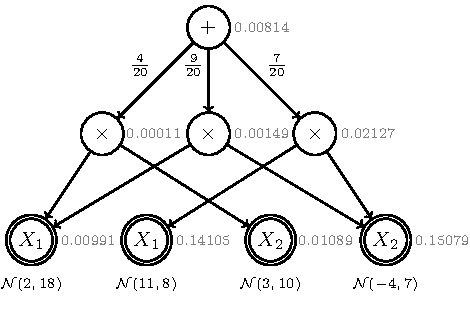
\includegraphics{figures/spninference.pdf}}

  \caption[Marginal inference in a GSPN]{Inference of $\mathcal{S}(11, -4)$ in the SPN represented in Figure \ref{fig:gspn}. The approximate values of the nodes, computed in a bottom-up fashion, are on the right side of each node.}
  \label{fig:spninference}
\end{figure}

\section{SPNs as mixture models}
\label{sec:spn:trees}

\citet{Zhao2015} showed that any SPN is equivalent to a mixture of trees where each tree corresponds to a product of univariate distributions. Given an SPN $\mathcal{S}$ over $X_1, \cdots, X_n$, let $\mathcal{T} = (V_\mathcal{T}, E_\mathcal{T})$ be a subgraph of $\mathcal{S}$. $\mathcal{T}$ is called an \textbf{induced tree}\footnote{This notion has been used in the literature under different terms, e.g. \emph{induced tree} by \citet{Zhao2015}, \emph{parse tree} by \citet{Mei2017}, \emph{complete subnetwork} by \citet{Desana2016}, \emph{complete sub-circuit} by \citet{Chan2006, Dennis2015}.} from $\mathcal{S}$ if it can be constructed recursively, starting from the root node and then including all children of product nodes and exactly one child of sum nodes (with the corresponding edges). As proved by \citet[Theorems 1 and 2]{Zhao2015}, an induced tree $\mathcal{T}$ is an SPN, therefore $\mathcal{T}(\mathbf{X})$ represents a probability distribution. The density function of such distribution is given by:

\begin{equation}
  \mathcal{T}(\mathbf{x}) = \prod_{(u, v) \in E_\mathcal{T}} w(u, v) \prod_{j=1}^{n} T_j(x_j) \, ,
  \label{eq:inducedtree}
\end{equation}

\noindent where $w(u, v)$ is the weight of the edge $(u, v) \in E_\mathcal{T}$ if $u$ is a sum node or $1$ if $u$ is a product node; $T_j(X_j)$ is the probability distribution of a leaf of $\mathcal{T}$ ($\mathcal{T}$ contains $n$ leaves, one for each variable).

Let $\tau_\mathcal{S}$ denote the number of unique induced trees from $\mathcal{S}$, namely, its \textbf{network cardinality}, and $\mathcal{T}^i$ denote the $i$-th unique induced tree of $\mathcal{S}$. Then \citep[Theorem 4]{Zhao2015},

\begin{equation}
  \mathcal{S}(\mathbf{x}) = \sum_{i=1}^{\tau_\mathcal{S}} \mathcal{T}^i(\mathbf{x}) \, .
  \label{eq:mixture}
\end{equation}

\noindent This result is illustrated in Figure \ref{fig:inducedtrees}. The network cardinality of $\mathcal{S}$ depends on its structure and is exponential in the height of the SPN.

\begin{figure}
  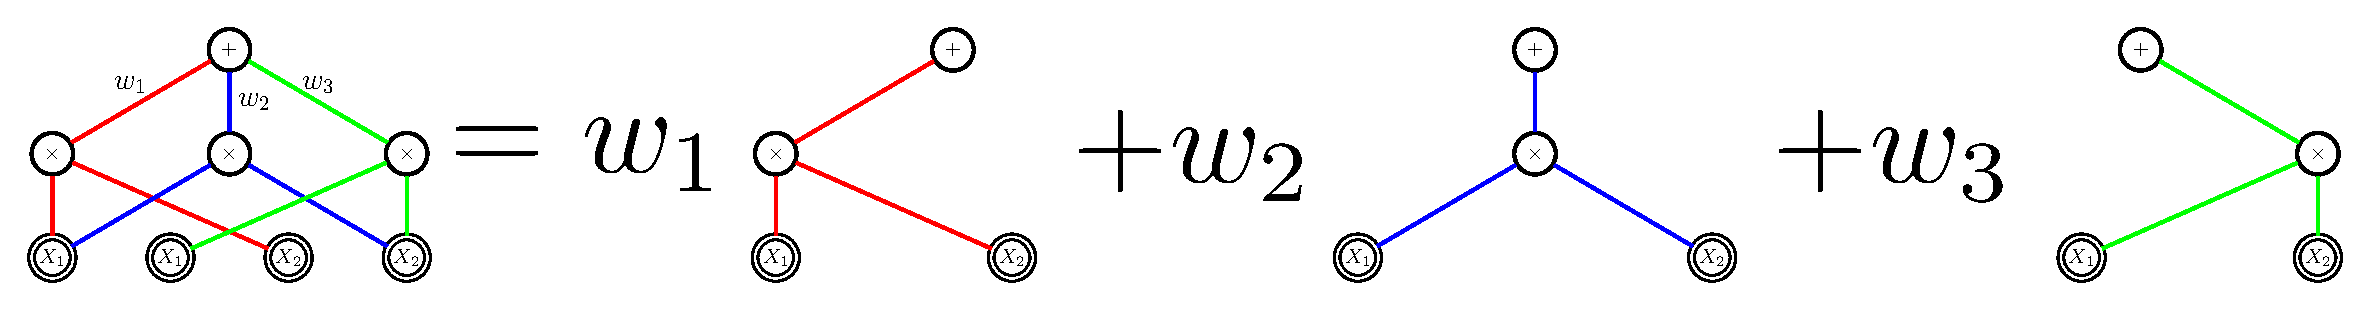
\includegraphics[width=\textwidth]{figures/inducedtrees.pdf}

  \caption[SPN as a mixture of induced trees]{An SPN as a mixture of induced trees. Source: \citet{Zhao2015}.}
  \label{fig:inducedtrees}
\end{figure}

\vspace{1em}

Given an SPN $\mathcal{S}$, from equations \ref{eq:inducedtree} and \ref{eq:mixture} we have:

\begin{equation}
  \label{eq:inducedtree_i}
  \mathcal{S}(\mathbf{x}) = \sum_{i=1}^{\tau_\mathcal{S}} w_i T^i(\textbf{x}) \, ,
\end{equation}

\noindent where $w_i := \prod_{(u, v) \in E_{\mathcal{T}_i}} w(u, v)$ and $T^i(\mathbf{x}) := \prod_{j=1}^n T^i_j(x_j)$ for all $i = 1, \cdots, \tau_\mathcal{S}$ (we are just splitting $\mathcal{T}_i$).

Let $Z$ be the latent variable that corresponds to the mixture, i.e., $\mathcal{S}(\mathbf{x} \mid z) = T^z(\textbf{x})$, and let $x_k, \cdots, x_l$ be values of RVs in $\mathbf{X}$. Then, for all $z \sim Z$,

\begin{eqnarray}
  \mathcal{S}(x_k, \cdots, x_l \mid z) & = & T^z(x_k, \cdots, x_l) \\
  & = & \prod_{j=1}^n T^z_j(x_k, \cdots, x_l) \\
  & = & T^z_k(x_k) \cdots T^z_l(x_l) \\
  & = & \mathcal{S}(x_k \mid z) \cdots \mathcal{S}(x_l \mid z) \, ,
\end{eqnarray}

\noindent which implies that the (observable) variables are independent given the mixture.

\vspace{1em}

If $\mathcal{S}$ is a GSPN, then $T^z(\mathbf{X})$ is a PDF formed by the product of the PDFs of independent Gaussian RVs. Thus, $T^z(\mathbf{X})$ is a multivariate Gaussian distribution with a diagonal covariance matrix. Therefore, a GSPN represents a GMM, where in each component the variables are uncorrelated.

However, GSPNs have an exponential network cardinality (with respect to the height of the network); therefore, they represent GMMs with a huge number of components. Despite the components share some parameters, this makes GSPNs much more expressive than typical learned GMMs while still remaining computationally tractable.

\section{Learning SPNs}
\label{sec:spn:learning}

SPNs are typically learned from data, and there exist various methods to accomplish this \citep{Peharz2015}. While recently, a variety of random methods that waive the necessity of structure learning have gained popularity \citep{Peharz2020, Geh2021}, in this section, we will focus on reviewing the most classical one -- LearnSPN. Our aim is not to delve too deeply into the topic of learning SPNs, but rather to gain a better understanding of the structure of the SPNs used in our experiments and the influence of learning parameters on these SPNs.

\textbf{LearnSPN}, the most classical schema used to learn SPNs \citep{Gens2013}, operates through a top-down divide-and-conquer approach that can learn both the structure (the underlying graph) and the parameters (weights and distributions at the leaves) of an SPN. To achieve this, it recursively splits the training set matrix into matrices with fewer instances or fewer variables, as shown in Figure \ref{fig:learnspn}. A high-level summary of the LearnSPN algorithm is presented in Algorithm \ref{alg:learnspn}.

\begin{figure}
  \centering
  \scalebox{0.3}{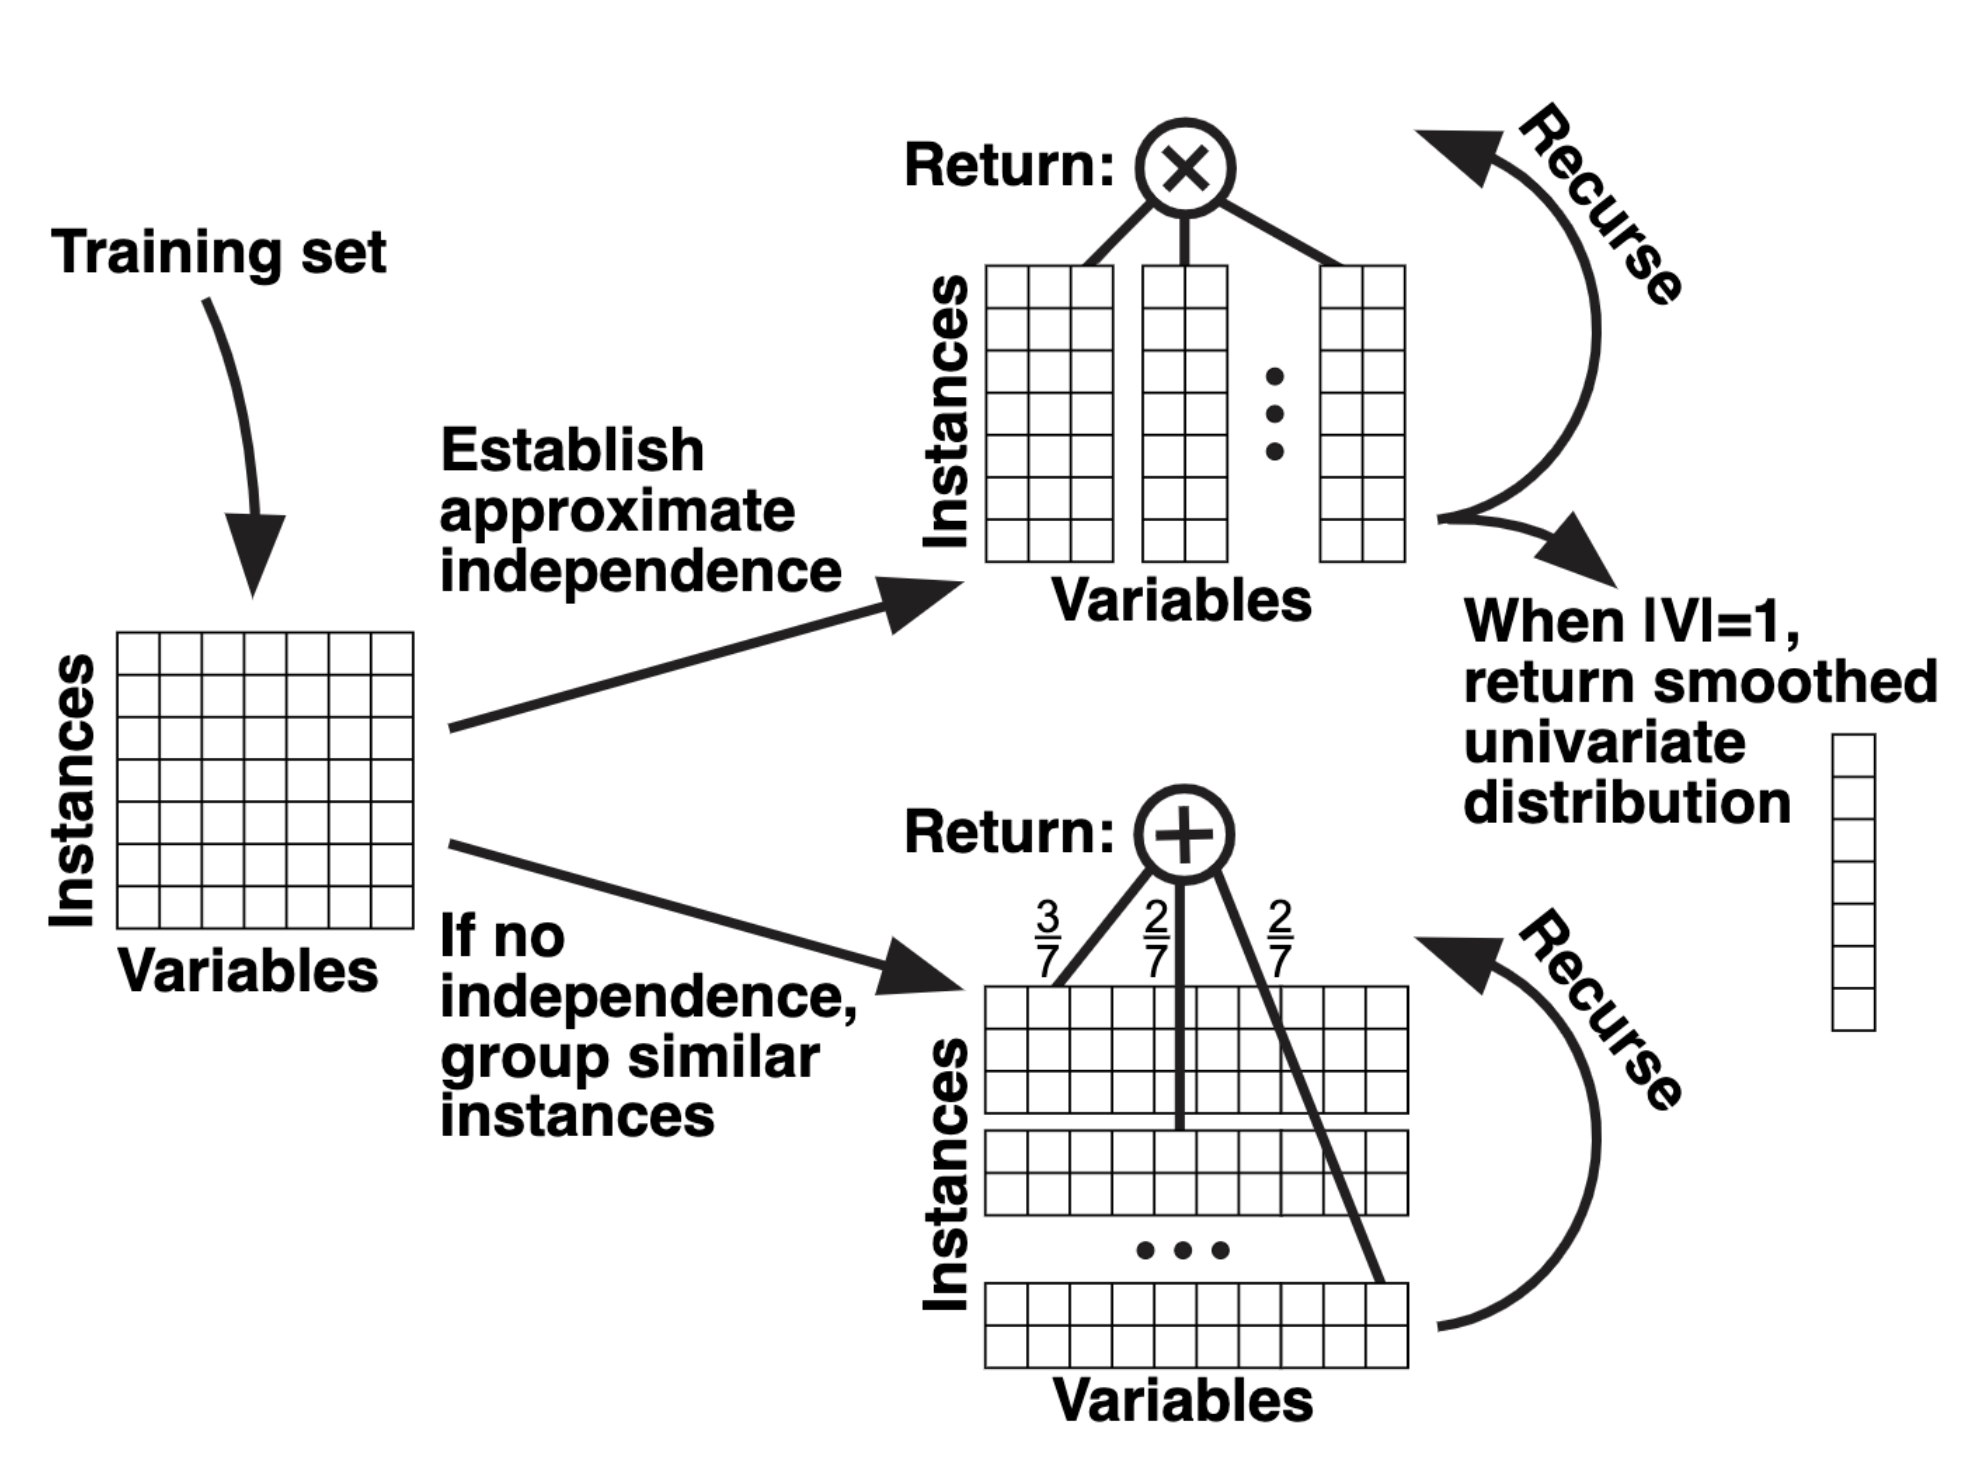
\includegraphics{figures/learnspn.png}}

  \caption[LearnSPN schema]{Illustration of LearnSPN algorithm. Source: \citet{Gens2013}.}
  \label{fig:learnspn}
\end{figure}

\begin{algorithm}[h]
  \caption{LearnSPN schema}
  \label{alg:learnspn}
  \begin{algorithmic}
    \Input{set of instances $D$ and set of variables $V$}
    \Output{an SPN representing a distribution over $V$ learned from $D$}
  \end{algorithmic}
  \begin{algorithmic}[1]
    \If{$|V| = 1$}
    \State \Return{univariate distribution estimated from the variable's values in $D$}
    \Else
    \LineComment{Try to partition $V$ into approximately independent subsets $V_j$.} \label{alg:learnspn:prod}
    \If{partition is successful}
    \State \Return{product node pointing to all $\textrm{LearnSPN}(D, V_j)$}
    \Else
    \LineComment{Partition $D$ into subsets of similar instances $D_i$.} \label{alg:learnspn:sum}
    \State \Return{sum node pointing to all $\textrm{LearnSPN}(D_i, V)$ with weights $\frac{|D_i|}{|D|}$}
    \EndIf
    \EndIf
  \end{algorithmic}
\end{algorithm}

The specificities for partitioning a variable set $V$ into approximately independent subsets $V_j$ (line \ref{alg:learnspn:prod}) and partitioning a dataset $D$ into subsets of similar instances $D_i$ (line \ref{alg:learnspn:sum}) were intentionally left vague by \citet{Gens2013}, making LearnSPN more of a schema than a single algorithm.

It is important to highlight that LearnSPN exclusively learns tree-shaped SPNs. Consequently, the resulting structures tend to be larger than if they were not constrained to trees. Furthermore, this implies that there is likely a considerable number of leaves associated with each variable.

There are different approaches to accomplish partitioning the dataset. One common method for finding approximately independent subsets of variables is the G-test \citep{Gens2013}. However, different implementations may employ different independence tests. For instance, the open-source library SPFlow \citep{Molina2019SPFlow} utilizes the Randomized Dependence Coefficient \citep{Lopes-Paz2013} as its default independence test.

To split instances, clustering methods can be employed, such as $k$-means \citep{MacQueen1967} and GMM clustering. Each of these methods requires specific hyperparameters. In LearnSPN implementations, it is typical to specify a threshold for determining variable independence, a minimum number of instances for partitioning, a desired number of clusters, and, in the case of learning GSPNs, a minimum variance for the Gaussian distributions in the leaves to prevent the learning of degenerate GSPNs.

The choice of hyperparameters has a significant impact on the size of learned SPNs.

\section{MAP inference}
\label{sec:spn:map}

SPNs are often built to solve structured prediction problems, where a solution is found by performing \textbf{Maximum-A-Posteriori} (MAP) inference in the model. MAP inference aims to find the most probable values for a set of RVs according to a probability distribution, and it is closely related to finding a global maximum in SPNs.

\begin{definition}[MAP Inference]
  Given a probability density function\footnote{We are assuming continuous RVs, but in the case of discrete RVs the definition is similar but uses a probability mass function instead of a probability density function.} $p(\mathbf{X})$, disjoint sets $\mathbf{X}^q$, $\mathbf{X}^0$, $\mathbf{X}^m$ such that $\mathbf{X} = \mathbf{X}^q \cup \mathbf{X}^0 \cup \mathbf{X}^m$, and an evidence $\mathbf{x}^0$ on $\mathbf{X}^0$, MAP inference consists of finding the most probable configuration for $\mathbf{X}^^q$ given $\mathbf{x}^0$ and ignoring (marginalizing) the RVs in $\mathbf{X}^m$, that is:

  \begin{equation}
    \label{eq:map}
    \MAP\left(p, \mathbf{X}^q, \mathbf{x}^0, \mathbf{X}^m\right) := \argmax_{\mathbf{x}^q \in \mathbb{R}^{|\mathbf{X}^q|}}{p\left(\mathbf{x}^q \mid \mathbf{x}^0\right)} \, .
  \end{equation}
\end{definition}

MAP inference is a generalization of Most Probable Explanation (MPE) inference, which consists in finding the most probable configuration for a set of RVs $\mathbf{X}^q$ given an evidence $\mathbf{x}^0$ (without a set of RVs to marginalize), and is inherently harder than it in classical probabilistic graphical models (PGMs) like Bayesian Networks and Markov Networks \citep{Park2004}.

Equation \ref{eq:map} implies that:

\begin{eqnarray}
  \MAP\left(p, \mathbf{X}^q, \mathbf{x}^0, \mathbf{X}^m\right) & = & \argmax_{\mathbf{x}^q \in \mathbb{R}^{|\mathbf{X}^q|}}{p\left(\mathbf{x}^q, \mathbf{x}^0\right)} \\
  & = & \argmax_{\mathbf{x}^q \in \mathbb{R}^{|\mathbf{X}^q|}}{\int_\mathbb{R} \cdots \int_\mathbb{R} p\left(\mathbf{x}^q, \mathbf{x}^0, x^m_1, \cdots, x^m_k\right) dx^m_1 \cdots dx^m_k} \, .
\end{eqnarray}

The valuation $\MAP(\cdot)$ is named \textbf{MAP assignment} and the conditional probability $p(\MAP(\cdot) \mid \mathbf{x}^0)$ is named \textbf{MAP value}. In this work, we refer to the problem of performing MAP inference as \textbf{MAP problem}.

\vspace{1em}

Although marginal and conditional inference take linear time in SPNs, MAP inference is computationally difficult. In fact, it is proven to be $\mathcal{NP}$-Hard in discrete SPNs; distinct proofs are found in \citep{Peharz2015}, \citep{Peharz2016} and \citep{Conaty2017}. Moreover, \citet{Conaty2017} proved the non-approximability of MAP inference within a sublinear factor in discrete SPNs of height 2, as well as the non-approximability within any factor $2^{f(m)}$ for any sublinear function $f$ of the input size $m$ in discrete SPNs of height $\geq 3$, even if there is no evidence and if their structure is a tree. Their results are summarized in Table \ref{tab:mapcomplexity}.

\begin{table}
  \centering

  \begin{tabular}{ccc}
    \toprule
    \bfseries Height & \bfseries Lower bound & \bfseries Upper bound \\ \midrule
    $1$              & $1$                   & $1$                   \\
    $2$              & $(m-1)^\epsilon$      & $m-1$                 \\
    $\geq 3$         & $2^{s^\epsilon}$      & $2^s$                 \\
    \bottomrule
  \end{tabular}

  \caption[Lower and upper bounds on the approximation threshold for a polynomial-time algorithm for MAP inference in discrete SPNs]{Lower and upper bounds on the approximation threshold for a polynomial-time algorithm for MAP inference in discrete SPNs: $s$ denotes the size of the instance, $m$ is the number of internal nodes, $\epsilon$ is a non-negative number less than $1$. Source: \citet{Conaty2017}.}
  \label{tab:mapcomplexity}
\end{table}

\subsection{Reduction from MAP to MAX}
\vspace{1em}

MAP inference splits the set of RVs $\mathbf{X}$ in three parts $\mathbf{X}^q$, $\mathbf{X}^0$, $\mathbf{X}^m$ such that $\mathbf{X} = \mathbf{X}^q \cup \mathbf{X}^0 \cup \mathbf{X}^m$. \citet{Mei2017} proved that every MAP problem can be reduced to a special case of MAP inference without evidence and RVs to marginalize ($\mathbf{X}^0 = \emptyset$, $\mathbf{X}^m = \emptyset$) in linear time in the size of the SPN. Formally, this reduced problem, which they called MAX inference, consists in computing:

\begin{equation}
  \MAX(p) := \argmax_{\mathbf{x}} p(\textbf{x}) \, ,
\end{equation}

\noindent that is, to find the global maximum of a PDF.

The transformation of a MAP problem to a MAX problem in linear time implies that any efficient algorithm for solving MAX inference can be used to efficiently solve MAP inference.

Given a MAP problem $\mathbf{X}^q, \mathbf{x}^0, \mathbf{X}^m$ over an SPN $\mathcal{S}$, the MAP2MAX algorithm developed by \citet{Mei2017} returns a new SPN $\mathcal{S}'$ over $\mathbf{X}^q$ such that $\mathcal{S}'(\mathbf{x}^q) = \mathcal{S}(\mathbf{x}^q, \mathbf{x}^0)$ for all $\mathbf{x}^q \in \mathbb{R}^{|\mathbf{X}^q|}$, which implies $\MAX(\mathcal{S}') = \MAP(\mathcal{S}, \mathbf{X}^q, \mathbf{x}^0, \mathbf{X}^m)$. A pseudocode is given in Algorithm \ref{alg:map2max}. It is slightly modified from the one in the original paper because \citet{Mei2017} considers SPNs with RV indicators at their leaves.

\begin{algorithm}[h]
  \caption{MAP2MAX}
  \label{alg:map2max}
  \begin{algorithmic}
    \Input{an SPN $\mathcal{S}$ over $\mathbf{X}$, an evidence $\mathbf{x}^0$, and a set $\mathbf{X^m}$ of RVs to marginalize}
    \Output{an SPN $\mathcal{S'}$ over $\mathbf{X}^q$ such that $\mathcal{S}'(\mathbf{x}^q) = \mathcal{S}(\mathbf{x}^q, \mathbf{x}^0)$}
  \end{algorithmic}
  \begin{algorithmic}[1]
    \LineComment Let $A$ be an auxiliary mapping from SPN nodes to real values.
    \ForAll{node $u$ of $\mathcal{S}$ in reverse topological order}
    \If{$u$ is a leaf with scope $X_i$}
    \If{$X_i \in \mathbf{X}^e$}
    \State $A_u \gets u(x^e_i)$
    \Else
    \State $A_u \gets -\infty$
    \EndIf
    \ElsIf{$u$ is a product node}
    \State $A_u \gets \prod_{v \in \ch(u)} A_v$
    \ElsIf{$u$ is a sum node}
    \ForAll{$v \in \ch(u)$}
    \State $w(u, v) \gets w(u, v) A_v$
    \EndFor
    \If{$\scope(u) \subseteq \mathbf{X}^e \cup \mathbf{X}^m$}
    \State $A_u \gets \sum_{v \in \ch(u)} w(u, v)$
    \Else
    \State{$A_u \gets 1$}
    \EndIf
    \EndIf
    \EndFor
    \ForAll{node $u$ of $\mathcal{S}$}
    \If{$\scope(u) \subseteq \mathbf{X}^e \cup \mathbf{X}^m$}
    \LineComment{Remove $u$ and the arcs/weights associated with $u$.}
    \EndIf
    \EndFor
    \State \Return{$\mathcal{S}$}
  \end{algorithmic}
\end{algorithm}

To be precise, the SPN resulting from MAP2MAX algorithm is not ``normalized,'' as the weights of arcs from sum nodes do not necessarily add up to 1 and therefore the resulting probability distribution is not normalized. However, SPNs can be normalized efficiently in linear time, as shown by \citet{Peharz2015}, and the normalization simply divides densities by a constant, not affecting the semantic of the model and its modes.

Since MAP inference can be reduced to MAX in linear time, we will assume, without loss of generality, that MAP inference in SPNs is seeking the solution to the MAX problem, which consists in simply finding a global maximum of a given distribution.

\subsection{Approximation algorithms}
\label{sec:map:approximate}

Table \ref{tab:mapcomplexity} shows that MAP inference in SPNs is not only hard to perform exactly, but also hard to approximate. Since the introduction of SPNs, different approximation algorithms have been proposed; first Max-Product \citep{Poon2011}, and then adaptations such as ArgMax-Product \citep{Conaty2017} and K-Best Tree \citep{Mei2017}.

\vspace{1em}

\textbf{Max-Product} is a greedy algorithm that runs in linear time and consists of, given an SPN $\mathcal{S}$:

\begin{enumerate}
  \item Build a Max-Product Network $\mathcal{M}$ from $\mathcal{S}$ by replacing all sum nodes with $\max$ nodes (which selects the maximum values among its children). Replace each leaf with the global maximum of its distribution.
  \item Compute the values of all nodes in $\mathcal{M}$ by visiting all nodes starting from the leaves, similar to the process of performing marginal inference in an SPN as seen in Algorithm \ref{alg:inference}.
\end{enumerate}

The pseudocode for Max-Product is given in Algorithm \ref{alg:maxproduct}.

\begin{algorithm}[h]
  \caption{Max-Product}
  \label{alg:maxproduct}
  \begin{algorithmic}
    \Input{an SPN $\mathcal{S}$ over $\mathbf{X}$}
    \Output{a valuation $\mathbf{x}$ for $\mathbf{X}$ that is an approximation of $\argmax_{\mathbf{x}} \mathcal{S}(\textbf{x})$}
  \end{algorithmic}
  \begin{algorithmic}[1]
    \LineComment{For any node $u$, let $A_u$ denote a mapping from RVs to values (initially empty).}
    \ForAll{node $u$ of $\mathcal{S}$ in reverse topological order}
    \If{$u$ is a leaf over $X_i$}
    \State $A_u \gets \{X_i: \argmax_{x} u(x)\}$ \Comment{e.g. for $u \sim \mathcal{N}(\mu, \sigma^2)$, $\argmax_{x} u(x) = \mu$}
    \State $M_u \gets u(A_u[X_i])$
    \ElsIf{$u$ is a product node}
    \State $A_u \gets \cup_{v \in \ch(u)} A_v$
    \State $M_u \gets \prod_{v \in \ch(u)} V_v$
    \ElsIf{$u$ is a sum node}
    \State $v^* \gets \argmax_{v \in \ch(u)} w_v M_v$ \label{alg:maxproduct:sum}
    \State $A_u \gets A_{v^*}$
    \State $M_u \gets w_{v^*} M_{v^*}$
    \EndIf
    \EndFor
    \State \Return{$A_\textrm{root}$}
  \end{algorithmic}
\end{algorithm}

\begin{figure}
  \centering
  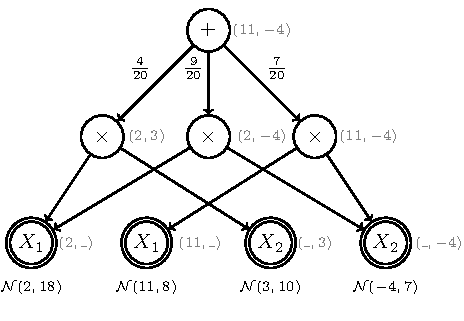
\includegraphics{figures/maxproduct.pdf}

  \caption[Illustration of Max-Product]{
    Max-Product algorithm in the GSPN shown in Figure \ref{fig:gspn}. On the right of each node $v$, the value of $\map_2(v)$ as computed by Max-Product. The algorithm outputs the configuration $X_1=11, X_2=-4$.
  }

  \label{fig:maxproduct}
\end{figure}

Figure \ref{fig:maxproduct} illustrates Max-Product algorithm finding a MAP assignment in the GSPN shown in Figure \ref{fig:gspn}.

This algorithm is called Best Tree by \citet{Mei2017} because it actually finds the induced tree of the SPN with the largest MAP value. \citet{Peharz2016} proved that it finds the exact solution of MAP inference in the subclass of selective SPNs\footnote{A sum node $u$ is \textbf{selective} if for all choices of weights $w$ and all possible $\mathbf{x}$ it holds that at most one child of $u$ is non-zero. An SPN is selective if all its sum nodes are selective.}, but that is not useful in the context of GSPNs which are not selective.

\vspace{1em}

\citet{Conaty2017} proposed a slightly modified version of Max-Product algorithm which they called \textbf{ArgMax-Product}. In the worst case scenario it achieves the same result of Max-Product, but reportedly perform significantly better in average. The idea is, for each sum node $u$, to compute the value of the sub-SPN rooted in $u$ for each of the possible MAP assignments obtained by its children. Instead of just choosing the maximum value of $w(u, v) A_v$ for all $v \in \ch(u)$ (line \ref{alg:maxproduct:sum}), it actually computes the entire value of $v$ for all the sets of values of RVs that arise from its children. The trade-off is complexity: ArgMax-Product does $|\ch(v)|$ bottom-up evaluations of the SPN on every sum node $v$ in the SPN, so it has quadratic time complexity.

\vspace{1em}

\citet{Mei2017} noted that, given an SPN $\mathcal{S}$, Max-Product algorithm finds the induced tree with the largest MAX value. Motivated by their empirical finding that in several cases the exact MAX solution is an induced tree with a large value, although not necessarily the largest, they proposed an algorithm to find the $K$ induced trees of $\mathcal{S}$ with the largest value --- namely, \textbf{K-Best Tree} (KBT). The algorithm is similar to Max-Product, but, instead of propagating up the maximum value from each node, it propagates the top $K$. The overall time complexity of KBT is $O(|\mathcal{S}| K \log{K})$. If $K = 1$, KBT reduces to Max-Product.


\chapter{Modal EM for GSPNs}
\label{cap:algorithm}

The direct application of Modal EM, as discussed in Chapter \ref{cap:gmm}, to SPNs is intractable due to the large number of components in the mixture, which corresponds to the number of induced trees in the SPN. To address this limitation, we devised an adaptation of Modal EM that leverages the recursive nature of SPNs.

Our contribution has been published in a conference \citep{Madeira2022}, but we have revised the notation to present it with more clarity in this chapter. Additionally, we will provide a proof of the ascending property of the algorithm (Theorem \ref{thm:alg_correctness}) which was not included in the paper.

In this chapter, we will first introduce Modal EM for GSPNs algorithm and show how it was constructed (Section \ref{sec:algorithm:intro}), then we will prove its correctness (Section \ref{sec:algorithm:proof}). Next, we will discuss two applications: MAP inference and clustering (Section \ref{sec:algorithm:applications}).

\section{The algorithm}
\label{sec:algorithm:intro}

\textbf{Modal EM for GSPNs} traverses the network from bottom to top, and each node propagates $2n$ values. Each iteration of it takes $\Theta\left(n|\mathcal{S}|\right)$, where $n$ is the number of RVs, and $|\mathcal{S}|$ is the number of nodes in the GSPN. The pseudo-code is presented in Algorithm \ref{alg:mem}.

\begin{algorithm}[h]
  \caption{Modal EM for GSPNs}
  \label{alg:mem}
  \begin{algorithmic}
    \Input{a GSPN $\mathcal{S}$ over $X_1, \cdots, X_d$ and a point $\mathbf{x}^{(r)} \in \mathbb{R}^d$}
    \Output{a point $\mathbf{x}^{(r+1)} \in \mathbb{R}^d$ such that $\mathcal{S}\left(\mathbf{x}^{(r+1)}\right) \geq \mathcal{S}\left(\mathbf{x}^{(r)}\right)$}
  \end{algorithmic}
  \begin{algorithmic}[1]
    \ForAll{node $u$ of $\mathcal{S}$ in reverse topological order}
    \If{$u$ is a leaf}
    \LineComment{Let $X_i$ be the RV in the scope of $u$;}
    \LineComment{Let $\mu$ and $\sigma$ be the parameters of the Gaussian of $u$.}
    \State $N^u_i \gets \frac{u\left(x^{(r)}_i\right)\mu}{\sigma^2}$,  $D^u_i \gets \frac{u\left(x^{(r)}_i\right)}{\sigma^2}$ \label{alg:mem:leaf:1}
    \ForAll{RV $X_j \neq X_i$}
    \State $N^u_j \gets D^u_j \gets u\left(x^{(r)}_i\right)$ \label{alg:mem:leaf:2}
    \EndFor
    \ElsIf{$u$ is a product node}
    \ForAll{RV $X_i$} \label{alg:mem:product}
    \State $N^u_i \gets \prod_{v \in \ch(u)} N^v_i$
    \State $D^u_i \gets \prod_{v \in \ch(u)} D^v_i$
    \EndFor
    \ElsIf{$u$ is a sum node}
    \ForAll{RV $X_i$} \label{alg:mem:sum}
    \State $N^u_i \gets \sum_{v \in \ch(u)} w(u, v) N^c_i$
    \State $D^u_i \gets \sum_{v \in \ch(u)} w(u, v) D^v_i$
    \EndFor
    \EndIf
    \EndFor
    \State \Return{$\frac{\mathbf{N}^\text{root}}{\mathbf{D}^\text{root}}$} \label{alg:mem:return}
  \end{algorithmic}
\end{algorithm}

We will now show how we constructed the algorithm.
If $\mathcal{S}(\mathbf{x})$ is the density of a GSPN, then $T^k(\mathbf{x})$ ($k = 1, \cdots, \tau$) corresponds to the multiplication of the densities in the leaves of its $k$-th induced tree, as seen in Section \ref{sec:spn:fundamentals}. Let $T^k_i\left(x_i\right)$ be the density of the leaf with scope $X_i$, $X_i \sim \mathcal{N}\left(\mu_{k_i}, \sigma^2_{k_i}\right)$, in the $k$-th induced tree. Then:

\begin{equation}
  T^k(\mathbf{x}) = \prod_i^n T^k_i\left(x_i\right) \, ,
\end{equation}

\noindent where $n$ is the number of RVs in the SPN. Therefore, starting from Equation \ref{eq:mem:maximization}, we have:

\begin{eqnarray}
  \label{eq:mem:construction:start}
  \mathbf{x}^{(r+1)} & = & \arg\max_\mathbf{x} \sum_k q_k \left( \log{\prod_i T^k_i(x_i)} \right) \\
  & = & \arg\max_\mathbf{x} \sum_k q_k \left(\sum_i \log{T^k_i(x_i)} \right) \\
  & = & \arg\max_\mathbf{x} \sum_k \sum_i \left(q_k \log{T^k_i(x_i)} \right) \\
  & = & \times_i \arg\max_{x_i} \sum_k \left(q_k \log{T^k_i(x_i)} \right).
\end{eqnarray}

The last equation above states that each coordinate of the $\mathbf{x}^{(r+1)}$ vector is obtained separately, by maximizing only over the corresponding dimension $\mathbf{x}^{(r+1)}_i$. Hence, for a fixed $i$, we only need to find $x_i$ that maximizes $g(x_i) := \sum_k q_k \log{T^k_i(x_i)}$.

The logarithm of the probability density function $f(x)$ of a univariate Gaussian distribution with mean $\mu$ and variance $\sigma^2$ is:

\begin{equation}
  l(x) = \log{f(x)} = -\log(\sigma) - \frac{1}{2} \log(2\pi) - \frac{(x-\mu)^2}{2\sigma^2} \, .
\end{equation}

The first and second derivatives of that function are, respectively:

\begin{equation}
  l'(x)  =  \frac{\mu - x}{\sigma^2}, \text{ and }
  l''(x)  =  -\frac{1}{\sigma^2} \, .
\end{equation}

\noindent That implies that $g(x_i)$ is a sum of quadratic functions with negative second derivative, therefore it has exactly one maximum. Its derivative is:

\begin{equation}
  g'(x_i) = \sum_k^\tau \left( q_k \frac{\mu_{k_i} - x_i}{\sigma_{k_i}^2} \right) \, .
\end{equation}

\noindent Thus, to compute $x^{(r+1)}_i = \arg\max_{x_i} g(x_i)$ we can calculate the point where it is zero. By solving $g'(x_i) = 0$, using Equation \ref{eq:mem:expectation} to find the value of $q_k$, we get:

\begin{equation} \label{eq:memfraction}
  x^{(r+1)}_i = \frac{\sum_k^\tau \frac{q_k \mu_{k_i}}{\sigma_{k_i}^2}}{\sum_k^\tau \frac{q_k}{\sigma_{k_i}^2}}
  = \frac{\sum_k^\tau \frac{w_k T^k\left(\mathbf{x}^{(r)}\right) \mu_{k_i}}{\mathcal{S}\left(\mathbf{x}^{(r)}\right) \sigma_{k_i}^2}}{\sum_k^\tau \frac{w_k T^k\left(\mathbf{x}^{(r)}\right)}{\mathcal{S}\left(\mathbf{x}^{(r)}\right) \sigma_{k_i}^2}}
  =   \frac{\sum_k^\tau \frac{\mu_{k_i}}{\sigma_{k_i}^2} w_k T^k\left(\mathbf{x}^{(r)}\right)}{\sum_k^\tau \frac{1}{\sigma_{k_i}^2} w_k T^k\left(\mathbf{x}^{(r)}\right)} \, .
\end{equation}

\noindent Note that this equation is equivalent to Equation \ref{eq:mem:gmm} (just indexed by $i$), demonstrating the equivalence of the iterative schema proposed by \citet{Carreira-Perpinan2000} and Modal EM as proposed by \citet{Li2007}. This iterative scheme has been shown to be equivalent to a generalized Mean-Shift algorithm by \citet{Chacon2019}, establishing a relation between Modal EM and Mean-Shift.

We aim to efficiently compute the value of each $i$-th random variable in the GSPN using our algorithm. Note that the numerator and denominator of the fraction in Equation \ref{eq:memfraction} are similar to the evaluation of the GSPN in $\mathbf{x}^{(r)}$, which can be expressed as $\mathcal{S}(\mathbf{x}^{(r)}) = \sum_k^\tau w_k T^k(\mathbf{x}^{(r)})$. However, there is a constant factor multiplying $w_k$ in both cases, which depends on the parameters of the leaf node of the $i$-th random variable in the $k$-th induced tree. This factor is $\frac{\mu_{k_i}}{\sigma^2_{k_i}}$ for the numerator and $\frac{1}{\sigma^2_{k_i}}$ for the denominator.

So, to compute the value of each RV, our algorithm performs a bottom-up evaluation of the GSPN and propagates $2n$ values for each node. For each random variable, one value is computed for the numerator (stored in $N$) and other for the denominator (stored in $D$) of Equation \ref{eq:memfraction}. Finally, we divide the vectors ($N$ by $D$) to get $\mathbf{x}^{(r+1)}$.

\section{Proof of correctness}
\label{sec:algorithm:proof}

We will now demonstrate, in Theorem \ref{thm:alg_correctness}, that our algorithm implements Modal EM and, therefore, is ascending. To accomplish that we will use Lemma \ref{lem:alg_computation}, which formalizes the argument given in the end of the construction of the algorithm in Section \ref{sec:algorithm:intro}.

\begin{lemma}
  \label{lem:alg_computation}
  For any node $u$ and any RV $X_i$ of a GSPN, Algorithm \ref{alg:mem} assigns the following values for $N^u_i$ and $D^u_i$:

  \begin{itemize}
    \item If $X_i$ is in the scope of $u$:

          \begin{equation}
            N^u_i = \sum_k^{\tau_u} \frac{\mu_{k_i}}{\sigma_{k_i}^2} w_k T_u^k\left(\mathbf{x}^{(r)}\right), \text{ and }
            D^u_i = \sum_k^{\tau_u} \frac{1}{\sigma_{k_i}^2} w_k T_u^k\left(\mathbf{x}^{(r)}\right) \, ,
          \end{equation}

          \noindent where $\tau_u$ denotes the number of induced trees of the SPN rooted on $u$ and $T_u^k(\mathbf{x}^{(r)})$ denotes the density of the assignment $\mathbf{x}^{(r)}$ in the $k$-th induced tree of the SPN rooted on $u$.

    \item If $X_i$ is not in the scope of $u$:

          \begin{equation}
            N^u_i = D^u_i = u\left(\mathbf{x}^{(r)}\right) \, .
          \end{equation}
  \end{itemize}
\end{lemma}

\begin{proof}
  Let $u$ be a node of a GSPN $\mathcal{S}$. Then $u$ must be either a univariate Gaussian node, a sum node or a product node. Proceed by cases.

  \begin{description}
    \item[Case 1:]
      Assume that $u$ is the univariate Gaussian distribution $\mathcal{N}(\mu, \sigma^2)$ over the RV $X_i$. Then, $\tau_u = 1$, $w_1 = 1$ and $T_u^1\left(\mathbf{x}^{(r)}\right) = u\left(x^{(r)}_i\right)$. Let $j$ be the index of RV $X_j$ in the scope of $\mathcal{S}$. If $j = i$, then line \ref{alg:mem:leaf:1} of the algorithm makes:

      \begin{eqnarray}
        N^u_i \gets & \frac{u\left(x^{(r)}_i\right)\mu}{\sigma^2} & = \sum_{k}^{\tau_u} \frac{\mu}{\sigma^2} w_k T_u^k\left(\mathbf{x}^{(r)}\right), \text{ and } \\
        D^u_i \gets & \frac{u\left(x^{(r)}_i\right)}{\sigma^2} & = \sum_{k}^{\tau_u} \frac{1}{\sigma^2} w_k T_u^k\left(\mathbf{x}^{(r)}\right) \, ,
      \end{eqnarray}

      \noindent and if $j \neq i$, then line \ref{alg:mem:leaf:2} of the algorithm makes:

      \begin{equation}
        N^u_j \gets D^u_j \gets u\left(\mathbf{x}^{(r)}\right) \, ,
      \end{equation}

      \noindent as we wanted to show.

    \item[Case 2:] Assume that $u$ is a product node pointing to nodes $v \in \ch(u)$. Assume, by induction, that the result holds for all $v$. The loop in line \ref{alg:mem:product} of the algorithm assigns, for all $X_i$:

      \begin{equation}
        N^u_i \gets \prod_{v \in \ch(u)} N^v_i, \text{ and }
        D^u_i \gets \prod_{v \in \ch(u)} D^v_i \, .
      \end{equation}

      Fix a variable $X_i$. Then $X_i$ is in the scope of $u$ or not. If it is, it is in the scope of one (and only one) $v \in \ch(u)$ (recall that, by definition, a product node points to nodes with disjoint scopes).

      If $X_i$ is in not in the scope $u$, then, by induction:

      \begin{equation}
        N^u_i \gets \prod_{v \in \ch(u)} v\left(\mathbf{x}^{(r)}\right) = u\left(\mathbf{x}^{(r)}\right)\, ,
      \end{equation}

      as we wanted to show. If $X_i$ is in the scope of a $v^* \in \ch(u)$, fix $v^*$. Then, again by induction:

      \begin{equation}
        N^u_i \gets \prod_{v \in \ch(u) \setminus \{v^*\}} v\left(\mathbf{x}^{(r)}\right) \left( \sum_k^{\tau_{v^*}} \frac{\mu_{k_i}}{\sigma_{k_i}^2} w_k T_{v^*}^k\left(\mathbf{x}^{(r)}\right) \right) \, .
      \end{equation}

      By the definition of induced tree (Equation \ref{eq:inducedtree_i}), we can untangle $v(\mathbf{x}^{(r)})$ to get:

      \begin{equation}
        N^u_i \gets \prod_{v \in \ch(u) \setminus \{v^*\}} \left( \sum_k^{\tau_{v}} w_k T_v^k\left(\mathbf{x}^{(r)}\right) \right) \left( \sum_k^{\tau_{v^*}} \frac{\mu_{k_i}}{\sigma_{k_i}^2} w_k T_{v^*}^k\left(\mathbf{x}^{(r)}\right) \right) \, .
      \end{equation}

      This combination of the induced trees of all children of $u$ produces:

      \begin{equation}
        N^u_i \gets \sum_k^{\tau_u} \frac{\mu_{k_i}}{\sigma_{k_i}^2} w_k T_u^k\left(\mathbf{x}^{(r)}\right) \, .
      \end{equation}

      The arguments for $D^k_i$ are analogous and are omitted for brevity.

    \item[Case 3:] Assume that $u$ is a sum node pointing to nodes $v \in \ch(u)$. Assume, by induction, that the result holds for all $v$. The loop in line \ref{alg:mem:sum} of the algorithm assigns, for all $X_i$:

      \begin{equation}
        N^u_i \gets \sum_{v \in \ch(u)} w(u, v) N^v_i, \text{ and }
        D^u_i \gets \sum_{v \in \ch(u)} w(u, v) D^v_i \, .
      \end{equation}

      Suppose that $X_i$ is in the scope of $u$. Then, by definition, it is in the scope of $v$ for all $v \in \ch(u)$. By induction, we have:

      \begin{equation}
        N^u_i \gets \sum_{v \in \ch(u)} \left( w(u, v) \sum_k^{\tau_v} \frac{\mu_{k_i}}{\sigma_{k_i}^2} w_k T_v^k\left(\mathbf{x}^{(r)}\right) \right) \, .
      \end{equation}

      By the definition of induced tree, that means:

      \begin{equation}
        N^u_i \gets \sum_k^{\tau_u} \frac{\mu_{k_i}}{\sigma_{k_i}^2} w_k T_u^k\left(\mathbf{x}^{(r)}\right) \, ,
      \end{equation}

      \noindent as we wanted to show.

      Now suppose that $X_i$ is not in the scope of $u$. Then, it is also not in the scope of $v$ for all $v \in \ch(u)$ and, by induction, we have:

      \begin{equation}
        N^u_i \gets \sum_{v \in \ch(u)} w(u, v) v\left(\mathbf{x}^{(r)}\right) \, ,
      \end{equation}

      \noindent which, by definition, is equal to:

      \begin{equation}
        N^u_i \gets u\left(\mathbf{x}^{(r)}\right) \, .
      \end{equation}

      The arguments for $D^k_i$ are analogous and are omitted for brevity.
  \end{description}
\end{proof}

\begin{theorem}
  \label{thm:alg_correctness}
  Modal EM for GSPNs (Algorithm \ref{alg:mem}) computes $\mathbf{x}^{(r+1)}$ from $\mathbf{x}^{(r)}$ such that $\mathcal{S}\left(\mathbf{x}^{(r+1)}\right) > \mathcal{S}\left(\mathbf{x}^{(r)}\right)$, unless $\mathbf{x}^{(r)}$ corresponds to a local maximum, in which case we have $\mathcal{S}\left(\mathbf{x}^{(r+1)}\right) = \mathcal{S}\left(\mathbf{x}^{(r)}\right)$.
\end{theorem}

\begin{proof}
  Fix $r$. The algorithm (line \ref{alg:mem:return}) returns $\mathbf{x}^{(r+1)} = \frac{N^\text{root}}{D^\text{root}}$. By Lemma \ref{lem:alg_computation},

  \begin{equation}
    N^\text{root}_i = \sum_k^{\tau} \frac{\mu_{k_i}}{\sigma_{k_i}^2} w_k T^k\left(x^{(r)}_i\right), \text{ and }
    D^\text{root}_i = \sum_k^{\tau} \frac{1}{\sigma_{k_i}^2} w_k T^k\left(x^{(r)}_i\right) \, .
  \end{equation}

  \noindent Hence, it returns the following coordinates for $\mathbf{x}^{(r+1)}$:

  \begin{equation}
    x_i^{(r+1)} = \frac{\sum_k^{\tau} \frac{\mu_{k_i}}{\sigma_{k_i}^2} w_k T^k\left(x^{(r)}_i\right)}{\sum_k^{\tau} \frac{1}{\sigma_{k_i}^2} w_k T^k\left(x^{(r)}_i\right)} \, .
  \end{equation}

  The construction depicted from Equation \ref{eq:mem:construction:start} to Equation \ref{eq:memfraction} shows that this value is equal to the one in Equation \ref{eq:mem:maximization}. Therefore, the algorithm computes the same value of Modal EM as developed by \citet{Li2007}. By the proof in Appendix A of \citep{Li2007}, $\mathcal{S}\left(\mathbf{x}^{(r+1)}\right) \geq \mathcal{S}\left(\mathbf{x}^{(r)}\right)$. By Theorem 1 of \citep{Wu1983}, the algorithm converges to a local maximum.
\end{proof}

In Section \ref{sec:algorithm:applications}, we will discuss some applications of Modal EM for GSPNs. In Chapter \ref{cap:experiments}, we will show it performs in practice.

\section{Applications}
\label{sec:algorithm:applications}

In this section, we will explore some potential applications of finding the modes of GSPNs in Maximum-A-Posteriori (MAP) Inference and modal clustering.

\subsection{MAP inference}

The greedy algorithms for MAP inference in SPNs discussed in Chapter \ref{cap:spn} are restricted to considering solutions derived solely from the modes of the distributions at the leaves. Consequently, these algorithms are not well-suited for accurately locating maxima of continuous SPNs, especially when the SPN contains maxima that are not maxima of the components of the mixture. Examples of such mixtures are depicted in Figures \ref{fig:amendola} and \ref{fig:gspn}. This limitation persists even in one dimension, as demonstrated by constructing a straightforward univariate GSPN comprising three nodes:

\begin{example}
  Consider a univariate GMM $X \sim 0.5 \mathcal{N}(1, 9) + 0.5 \mathcal{N}(3, 9)$. The PDF of such distribution is depicted in Figure \ref{fig:shortcomings}(a). An SPN representing this distribution can be constructed by connecting a sum root with two Gaussian leaves with weights 0.5 for both arcs, as shown in Figure \ref{fig:shortcomings}(b). The maximum of this PDF is located at $X = 2$ ($p(2) \approx 0.125$), which cannot be found by the approximation algorithms presented above that only explore solutions arising from the modes of the distributions at the leaves. These algorithms can only find $X = 1$ or $X = 3$ ($p(1) = p(3) \approx 0.119$).
\end{example}

\begin{figure}
  \begin{minipage}{0.5\textwidth}
    \centering
    \scalebox{0.55}{
      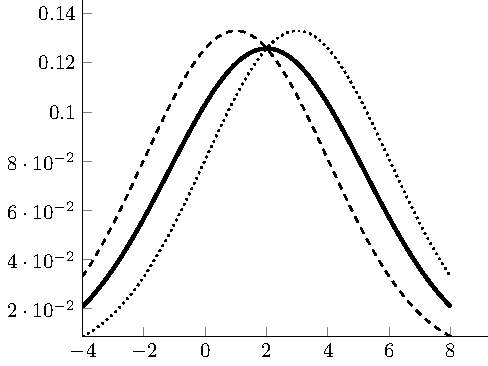
\includegraphics{figures/shortcomings-a.pdf}
    }

    (a)
  \end{minipage}\begin{minipage}{0.5\textwidth}
    \centering
    \scalebox{1.1}{
      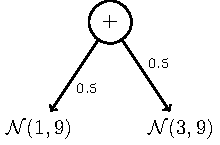
\includegraphics{figures/shortcomings-b.pdf}
    }

    (b)
  \end{minipage}

  \caption[Univariate GSPN in which Max-Product can not find MAP]{
    \textbf{(a)} Plot of the PDFs of three distributions: $X \sim \mathcal{N}(1, 9)$ (dashed line); $X \sim \mathcal{N}(3, 9)$ (dotted line); $X \sim 0.5 \mathcal{N}(1, 9) + 0.5 \mathcal{N}(3, 9)$ (solid line).
    \textbf{(b)} GSPN representing the distribution plotted as a solid line in (a). The approximation algorithms based on Max-Product, seen in Section \ref{sec:map:approximate}, are unable to find its unique mode, $X = 2$.
  }
  \label{fig:shortcomings}
\end{figure}

A common approach to enhance the approximate solutions obtained by these algorithms in discrete SPNs is to perform a \textbf{local search} in the space of possible assignments \citep{Maua2020}. This method involves iteratively modifying individual variable assignments to improve an existing solution. While this approach is straightforward for variable indicators or categorical random variables, adapting it to continuous SPNs, like GSPNs, could involve employing a hill-climbing method such as Modal EM. To illustrate this, Example \ref{ex:shortcomings} shows the application of Modal EM to the SPNs in Figures \ref{fig:shortcomings} and \ref{fig:gspn}.

\begin{example}
  \label{ex:shortcomings}
  \textbf{(a)} Consider the univariate GSPN shown in Figure \ref{fig:shortcomings}. Suppose an approximation algorithm has found the MAP solution $X = 1$, denoted as $x^{(0)}$. By applying Modal EM iteratively, we can observe its convergence towards the mode of the model, the value $X = 2$:

  \begin{minipage}{0.45\textwidth}
    \begin{eqnarray*}
      x^{(0)} & = & 1 \, ; \\
      x^{(1)} & \gets & 1.88934389 \, ; \\
      x^{(2)} & \gets & 1.98770550 \, ; \\
      x^{(3)} & \gets & 1.99863394 \, ;
    \end{eqnarray*}
  \end{minipage}\begin{minipage}{0.45\textwidth}
    \begin{eqnarray*}
      x^{(4)} & \gets & 1.99984822 \, ; \\
      x^{(5)} & \gets & 1.99998314 \, ; \\
      x^{(6)} & \gets & 1.99999813 \, ; \\
      x^{(7)} & \gets & 1.99999979 \, .
    \end{eqnarray*}
  \end{minipage}

  \vspace{1.5em}

  \noindent \textbf{(b)} Now consider the bivariate GSPN shown in Figure \ref{fig:gspn}. Applying Modal EM starting from the solution found by the Max-Product illustration in Figure \ref{fig:maxproduct}, $\mathbf{X} = (11, -4)$, we get:

  \begin{minipage}{0.45\textwidth}
    \begin{eqnarray*}
      \mathbf{x}^{(0)} & = & (11, -4) \, ; \\
      \mathbf{x}^{(1)} & \gets & (10.6418764, -3.9869965) \, ; \\
      \mathbf{x}^{(2)} & \gets & (10.5730441, -3.9844986) \, ; \\
      \mathbf{x}^{(3)} & \gets & (10.5580160,  -3.9839568) \, ;
    \end{eqnarray*}
  \end{minipage}\begin{minipage}{0.45\textwidth}
    \begin{eqnarray*}
      \mathbf{x}^{(4)} & \gets & (10.5546503, -3.9838357) \, ; \\
      \mathbf{x}^{(5)} & \gets & (10.5538923, -3.9838086) \, ; \\
      \mathbf{x}^{(6)} & \gets & (10.5537214, -3.9838023) \, ; \\
      \mathbf{x}^{(7)} & \gets & (10.5536829, -3.9838009) \, .
    \end{eqnarray*}
  \end{minipage}

  \vspace{1.5em}
\end{example}

Another possible strategy to perform MAP inference in GSPNs is to run Modal EM starting from multiple initial points, aiming to identify the highest mode among several local modes. However, this approach would face challenges due to the large number of modes typically present in a GSPN, as discussed in Chapter \ref{cap:gmm}.

\subsection{Modal clustering}

Clustering techniques play a crucial role in various data analysis domains, finding applications in areas such as pattern recognition, image analysis, and machine learning. Typically, a cluster is considered a high-density region within the sample space that is well separated from other high-density regions.

The majority of clustering methods categorizes points in a dataset by mean of a distance function. Such methods proceed by selecting a partition of the dataset that optimizes a chosen objective function that favors small intra-cluster distance and large inter-cluster distance. For instance, the classical $k$-means algorithm repeatedly identifies $k$ cluster centers and assigns data points to the nearest cluster center, with the aim of minimizing the squared distances from the clusters \citep{MacQueen1967}.

More recently, an increasing number of researchers have emphasized the importance of more explicitly incorporating density modeling into clustering procedures \citep{Carlsson2013}. In this direction, \citet{Chacon2019} conducted a comparative study of two distinct density-based clustering approaches: mixture model clustering and clustering based on high-density regions. In the case of mixture model clustering, clusters are associated with mixture components centered at their centroids, as inferred from the learned mixture model. On the other hand, clustering based on high-density regions associates clusters with the local maxima of the mixture density, focusing on regions of elevated density within the mixture.

Mixture model clustering offers the ability to explore more complex scenarios compared to modal clustering when the true density aligns with the assumed class of mixture densities. However, when mixture modeling is primarily employed to approximate any density within the dense space of mixture densities, as is often the case with SPNs, the association between clusters and mixture components becomes less reliable, and in that sense modal clustering is a promising approach.

While LearnSPN utilizes hierarchical clustering to construct the network's structure, cluster analysis on learned SPNs remains a largely unexplored field. Modal EM allows us to perform clustering via mode identification using GSPNs by ascending from any given point to a mode, which is considered to be the representative (center) of a cluster.


\chapter{Experiments}
\label{cap:experiments}

In this chapter, we will present the experimental results obtained through the implementation of the algorithms discussed in this thesis.

Modal EM for GSPNs has been made open source and is available within Julia's RPCircuits.jl package\footnote{Available at \url{https://github.com/RenatoGeh/RPCircuits.jl}.}. Furthermore, all the code utilized for conducting the experiments presented in this chapter can be found publicly at \url{https://github.com/tmadeira/gspn}.

To learn SPNs from data, we utilized the LearnSPN implementation provided by the SPFlow library\footnote{Available at \url{https://github.com/SPFlow/SPFlow}.} \citep{Molina2019SPFlow}. Instance splitting was performed using GMM clustering, while variable splitting was accomplished using the Randomized Dependence Coefficient \citep{Lopes-Paz2013}.

We will commence by presenting the outcomes of hierarchical clustering experiments carried out on the MNIST dataset (Section \ref{sec:exp:mnist}), which were previously published in the proceedings of a conference \citep{Madeira2022}. Following that, we will illustrate image segmentation experiments (Section \ref{sec:exp:segmentation}), which constitute an expanded version of what was presented in a workshop \citep{Madeira2023}.

\section{Hierarchical clustering}
\label{sec:exp:mnist}

In their work, \citet{Li2007} introduced Modal EM as a method to performing semi-parametric clustering in GMMs. Recognizing the presence of multiple modes in GMMs, they extended the approach to hierarchical clustering by iteratively learning models from the modes discovered in previous iterations. The models they use are kernel density estimators with increasing bandwidths.

Building upon this concept, we demonstrated the application of hierarchical clustering to GSPNs in a published paper \citep{Madeira2022}, where we presented empirical results showcasing the iterative learning of new GSPNs from the modes identified by Modal EM in the preceding models. This iterative schema allows us to progressively construct simpler and smaller models using the modes of previously learned models, which can serve as a representative summary of both the data and the model. The approach is particularly relevant in the contexts of model compression. In this section we reproduce these results.

To illustrate the method, we utilized the widely-known MNIST database of handwritten digits. The dataset consists of 60,000 grayscale images of size 28x28, representing the digits 0--9 in the training set, along with 10,000 images in the test set. Each pixel in the images is represented by an integer value ranging from 0 to 255. In our experiments, we focused solely on the images corresponding to the digit 0 from the MNIST database, forming a subset referred to as MNIST-0. This subset comprises 5,923 images in the training set and 980 images in the test set.

\begin{table}
  \centering

  \begin{tabular}{crrrr}
    \toprule
    \bfseries Iteration & \bfseries Instances & \bfseries Nodes & \bfseries Clusters & \bfseries Log Avg. Likelihood \\ \midrule
    \textbf{1}          & 5,923               & 74,556          & 201                & ~7,707                        \\
    \textbf{2}          & 201                 & 7,851           & 10                 & ~3,438                        \\
    \bottomrule
  \end{tabular}

  \caption[SPNs learned from MNIST-0 training set]{SPNs learned from MNIST-0 training set at iteration 1 and modes found in the first iteration at iteration 2. For each iteration, the tables show the number of instances used to learn the model, the network size (given by the number of nodes in the SPN), the number of clusters as found by running Modal EM starting from every point in the training set, and the log of the average likelihood for the test set in the learned SPN. Source: \citet{Madeira2022}.}
  \label{tab:mnist}
\end{table}

Initially, we trained a GSPN using the MNIST-0 dataset. Subsequently, we applied our Modal EM algorithm to each data point in the training set, generating a collection of representative summaries which correspond to modes of the model. Data points that ``converge'' to the same mode are grouped into the same cluster. These modes form a new dataset, from which we learn a new GSPN. This iterative process continues until the number of modes reaches an acceptably small value. In our experiments, we observed that two iterations were adequate to obtain a reduced set of models/clusters.

The results are shown in Table \ref{tab:mnist}, which includes information about the size of the network and the logarithm of the average likelihood of the test set in the learned SPN. These metrics provide insights into the model's capability to accurately represent the examples in the test set. In Figure \ref{fig:mnist}, we visualize the hierarchical clustering obtained through the iterative process applied to the MNIST-0 dataset. For clarity, we omit the initial 5,923 instances from the training dataset and only display the modes identified by Modal EM in the first and second iterations. Remarkably, even in a network that is approximately 10\% of the size of the original network, the modes appear to be good representatives of the dataset's diversity.

\begin{figure}
  \centering
  \scalebox{0.18}{
    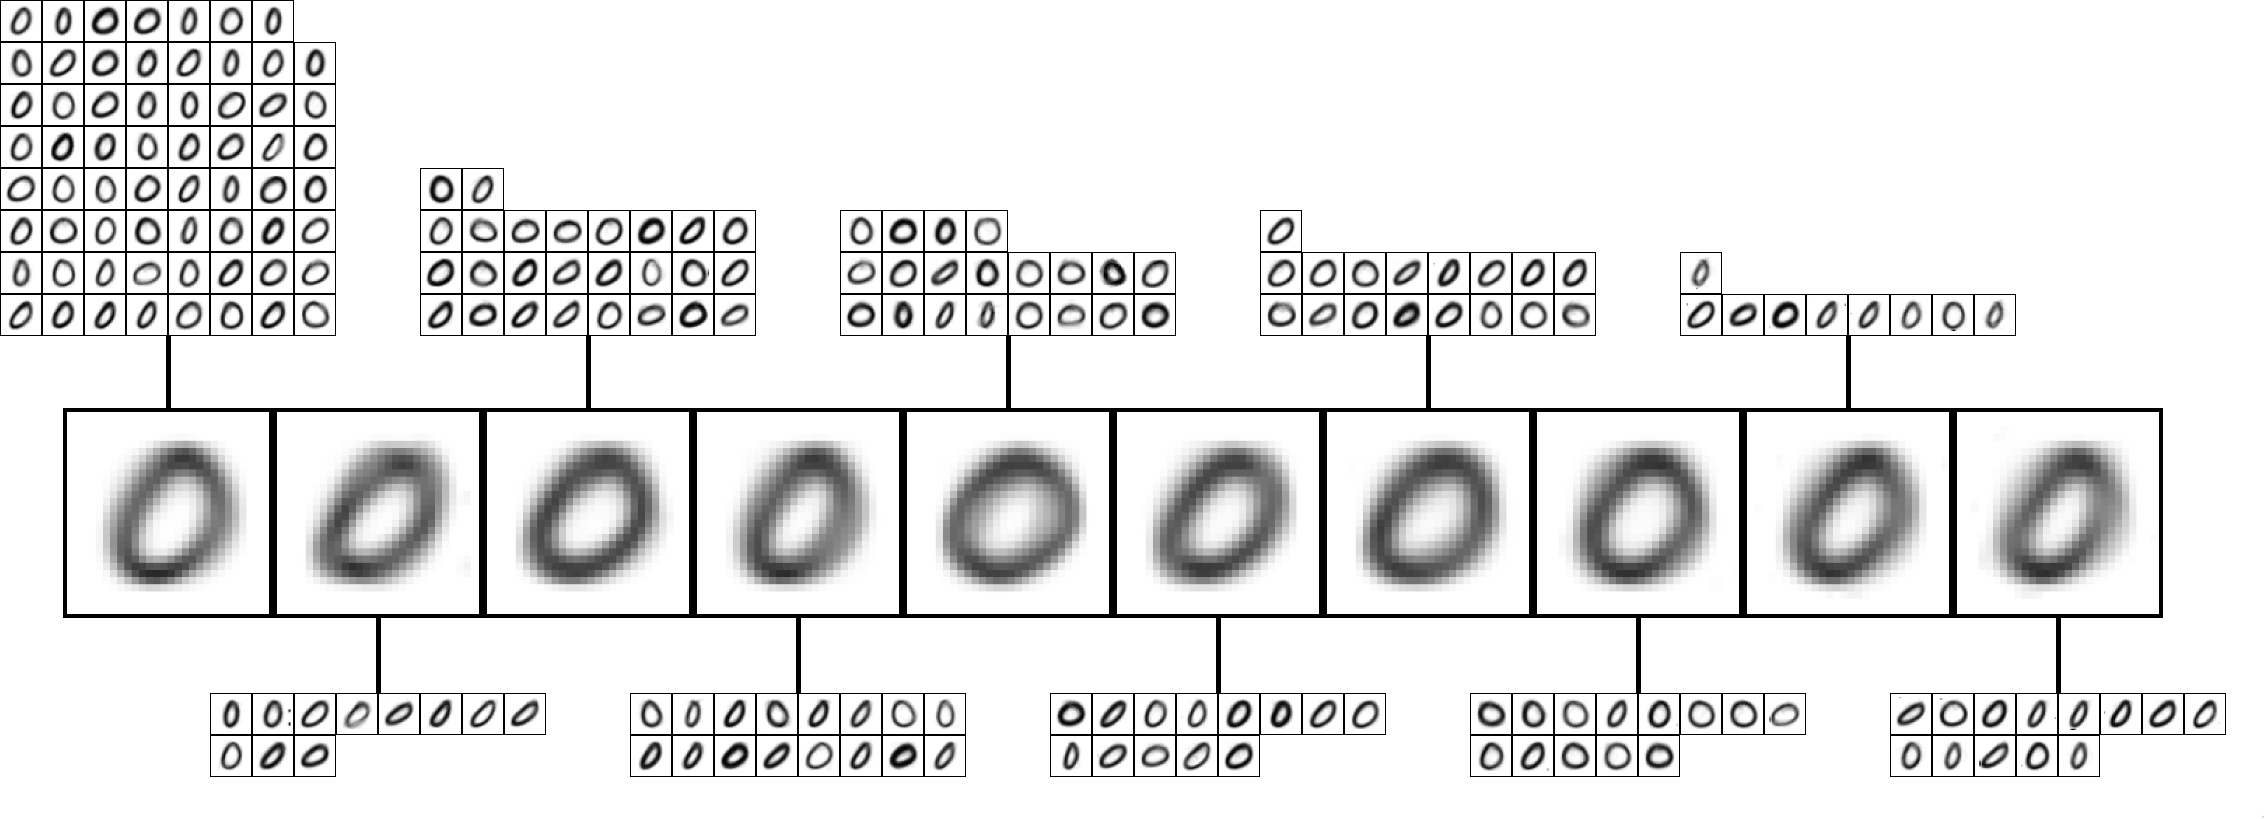
\includegraphics{figures/mnist.png}
  }
  \caption[Hierarchical clustering of MNIST-0 dataset]{Hierarchical clustering: Modes (representatives of the clusters) found in 2 iterations of Modal EM in GSPNs learned from MNIST-0 dataset. The smaller images correspond to the modes found in the first GSPN, the bigger ones correspond to the modes found in the second GSPN (learned from the modes from the first GSPN). Modes from the first GSPN are connected to their modes in the second GSPN. Source: \citet{Madeira2022}.}
  \label{fig:mnist}
\end{figure}

As noted in the paper, a limitation of this approach is that it tends to underrepresent high-density regions (large clusters) while overrepresenting low-density regions (small clusters) in the new dataset. To address this issue, one potential solution is to optimize for weighted log-likelihood in the structural and parametric learning algorithms. Another approach is to adjust the representation of models by over/undersampling them based on the density of their respective regions.

\section{Image segmentation}
\label{sec:exp:segmentation}

As another preliminary and visual investigation of the effectiveness of modal clustering on GSPNs, we performed some experiments with segmentation of the images depicted in Figure \ref{fig:segoriginals}.

\begin{figure}
  \centering

  \begin{minipage}{0.5\textwidth}
    \centering

    \scalebox{0.7}{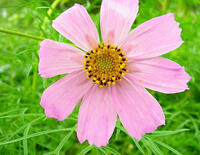
\includegraphics{figures/flower_200.jpg}}

    (a)
  \end{minipage}\begin{minipage}{0.5\textwidth}
    \centering

    \scalebox{0.7}{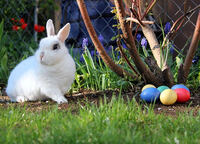
\includegraphics{figures/rabbit_200.jpg}}

    (b)
  \end{minipage}

  \vspace{0.5em}

  \begin{minipage}{0.5\textwidth}
    \centering

    \scalebox{0.7}{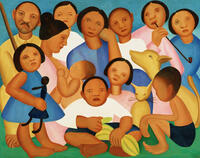
\includegraphics{figures/tarsila3_200.jpg}}

    (c)
  \end{minipage}\begin{minipage}{0.5\textwidth}
    \centering

    \scalebox{0.7}{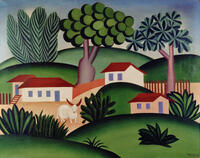
\includegraphics{figures/tarsila2_200.jpg}}

    (d)
  \end{minipage}

  \caption[Images used for segmentation (Flower, Easter Bunny, The Family, Landscape with Bull)]{Images used for segmentation. (a) Flower (200x155). (b) Easter Bunny (200x144). (c) Tarsila do Amaral's \emph{The Family} (200x158). (d) Tarsila do Amaral's \emph{Landscape with Bull} (200x158).}
  \label{fig:segoriginals}
\end{figure}

We generated datasets consisting of 5 variables by considering the RGB intensity values and $x$ and $y$ locations of each pixel from various images. The datasets were then used to learn GSPNs from data. We ran Modal EM starting from all the points in the dataset, finding the modes for which they converge. We considered that a cluster is formed by points that converge to the same mode. We then re-colored the image using the average color of the points in the cluster.

We experimented with different GSPNs by varying the minimum number of instances required for slicing in the learning process ($s$). Table \ref{tab:segstats} shows the number of nodes, network height and the number of clusters obtained for each GSPN when we vary $s$. One sees the great dependence between those quantities, as well as the quick increase in the number of modes when $s$ is smaller.

Figures \ref{fig:seg1} and \ref{fig:seg2} display a visual comparison of image segmentation by Modal EM in GSPNs and by the $k$-means algorithm as implemented by the scikit-learn library\footnote{Available at \url{https://scikit-learn.org}.}, where $k$ is set to the number of clusters identified by Modal EM trained with different $s$ hyperparameters.

Our results have shown satisfactory performance comparable to the widely-used $k$-means algorithm. However, visually, we observed that image segmentation using $k$-means with $k$ equivalent to the number of modes in the SPN yields more detailed segmentation results.

We conjecture that GSPN's slightly worse performance is due to a lack of fit to the model, which could be mitigated by changing the structure learning algorithm, performing fine-tuning of parameters or even using $k$-means solution as a initial model for refinements.

It is worth noting that image segmentation may not be the optimal application domain for SPNs, and also that GSPN modal clustering offers several advantages over traditional clustering techniques like $k$-means. It can effectively handle missing values, detect outliers based on probability thresholds, and easily scale up to handle more complex and high-dimensional domains.

\begin{table}
  \centering

  \begin{tabular}{crrrr}
    \toprule
    \bfseries Dataset   & \bfseries Parameter $s$ & \bfseries Nodes & \bfseries Height & \bfseries Clusters \\ \midrule
    Easter Bunny        & 20,000                  & 13              & 3                & 6                  \\
    Easter Bunny        & 15,000                  & 19              & 3                & 7                  \\
    Easter Bunny        & 10,000                  & 25              & 3                & 10                 \\
    Easter Bunny        & 5,000                   & 50              & 5                & 31                 \\
    Easter Bunny        & 2,000                   & 132             & 5                & 68                 \\
    Easter Bunny        & 500                     & 528             & 7                & 398                \\
    Easter Bunny        & 200                     & 1,267           & 9                & 676                \\ \midrule
    Flower              & 20,000                  & 13              & 3                & 2                  \\
    Flower              & 15,000                  & 19              & 3                & 5                  \\
    Flower              & 10,000                  & 25              & 3                & 8                  \\
    Flower              & 5,000                   & 61              & 3                & 27                 \\
    Flower              & 2,000                   & 155             & 5                & 79                 \\
    Flower              & 500                     & 595             & 5                & 228                \\
    Flower              & 200                     & 1,457           & 7                & 609                \\ \midrule
    The Family          & 20,000                  & 13              & 3                & 4                  \\
    The Family          & 15,000                  & 25              & 3                & 5                  \\
    The Family          & 10,000                  & 31              & 3                & 8                  \\
    The Family          & 5,000                   & 61              & 3                & 19                 \\
    The Family          & 2,000                   & 163             & 3                & 43                 \\
    The Family          & 500                     & 603             & 7                & 187                \\
    The Family          & 200                     & 1,504           & 7                & 555                \\ \midrule
    Landscape with Bull & 20,000                  & 13              & 3                & 6                  \\
    Landscape with Bull & 15,000                  & 25              & 3                & 12                 \\
    Landscape with Bull & 10,000                  & 31              & 3                & 15                 \\
    Landscape with Bull & 5,000                   & 55              & 3                & 24                 \\
    Landscape with Bull & 2,000                   & 145             & 3                & 38                 \\
    Landscape with Bull & 500                     & 563             & 7                & 255                \\
    Landscape with Bull & 200                     & 1,427           & 7                & 508                \\
    \bottomrule
  \end{tabular}

  \caption[Information about SPNs learned for image segmentation]{Information about SPNs learned for image segmentation.}
  \label{tab:segstats}
\end{table}

\newcommand{\segfigrow}[3]{
  \begin{minipage}{0.15\textwidth}
    \centering
    $s = #2$\\$k = #3$
  \end{minipage}    &
  \begin{minipage}{0.2\textwidth}
    \centering
    \scalebox{0.37}{\includegraphics{figures/fixed_mem_recolored_#1_200_#2_0.300000.png}}
  \end{minipage} &
  \begin{minipage}{0.2\textwidth}
    \centering
    \scalebox{0.37}{\includegraphics{figures/k_#3_recolored_#1_200.png}}
  \end{minipage}
}

\begin{figure}[p]
  \centering

  \begin{tabular}{ccc}
     & \bfseries GSPN & \bfseries $k$-means \\
    \segfigrow{flower}{20000}{2}            \\ \\
    \segfigrow{flower}{10000}{8}            \\ \\
    \segfigrow{flower}{2000}{79}            \\ \\
    \segfigrow{flower}{500}{228}            \\
  \end{tabular}

  \vspace{0.5em}

  (a)

  \vspace{2em}

  \begin{tabular}{ccc}
     & \bfseries GSPN & \bfseries $k$-means \\
    \segfigrow{rabbit}{20000}{6}            \\ \\
    \segfigrow{rabbit}{10000}{10}           \\ \\
    \segfigrow{rabbit}{2000}{68}            \\ \\
    \segfigrow{rabbit}{500}{398}            \\
  \end{tabular}

  \vspace{0.5em}

  (b)

  \caption[Image segmentation using GSPNs vs. $k$-means (Flower and Easter Bunny)]{Image segmentation using GSPNs vs. $k$-means. (a) Flower. (b) Easter Bunny.}
  \label{fig:seg1}
\end{figure}

\begin{figure}[p]
  \centering

  \begin{tabular}{ccc}
     & \bfseries GSPN & \bfseries $k$-means \\
    \segfigrow{tarsila3}{20000}{4}          \\ \\
    \segfigrow{tarsila3}{10000}{8}          \\ \\
    \segfigrow{tarsila3}{2000}{43}          \\ \\
    \segfigrow{tarsila3}{500}{187}          \\
  \end{tabular}

  \vspace{0.5em}

  (a)

  \vspace{2em}

  \begin{tabular}{ccc}
     & \bfseries GSPN & \bfseries $k$-means \\
    \segfigrow{tarsila2}{20000}{6}          \\ \\
    \segfigrow{tarsila2}{10000}{15}         \\ \\
    \segfigrow{tarsila2}{2000}{38}          \\ \\
    \segfigrow{tarsila2}{500}{255}          \\
  \end{tabular}

  \vspace{0.5em}

  (b)

  \caption[Image segmentation using GSPNs vs. $k$-means (The Family and Landscape with Bull)]{Image segmentation using GSPNs vs. $k$-means. (a) The Family. (b) Landscape with Bull.}
  \label{fig:seg2}
\end{figure}


\chapter{Final considerations}
\label{cap:final}

In this chapter, we will present the concluding remarks for this research. Section \ref{sec:final:summary} offers a concise summary of our work, emphasizing our contributions. Following that, Section \ref{sec:final:future} outlines potential avenues for future research in this domain.

\section{Summary}
\label{sec:final:summary}

This work investigated the problem of finding maxima of Gaussian Sum-Product Networks.

We reviewed literature about Gaussian Mixture Models, the number of local maxima in their probability density function, and techniques to find them. Additionally, we reviewed literature on Sum-Product Networks, their relationship with mixture models, and the challenges in finding optimal Maximum-A-Posteriori inference solutions in continuous SPNs.

We adapted the Modal EM schema from GMMs to GSPNs, creating a tractable fixed-point iteration algorithm capable of finding a mode in a GSPN from any arbitrary initial point. To the extent of our knowledge, this algorithm represents the first method specifically designed for mode-finding in GSPNs, making this work a modest but pioneering contribution in the study of modes in SPNs.

The correctness of the algorithm was proved, the time complexity was analyzed, and an implementation of it was released as open source in the RPCircuits.jl package.

After presenting the algorithm, we discussed some practical applications in MAP inference and cluster analysis. For MAP inference, we argued that Modal EM can be used to improve the solution of any existing algorithm, leading to an approach which provably finds a local optimum, a property most current algorithms lack.

For clustering, we performed illustrative examples on hierarchical clustering and image segmentation. For hierarchical clustering, we presented empirical results of iteratively learning smaller models starting from the training set of a digit from the MNIST dataset, and described how the approach can be used to categorize, explore or compress data. For image segmentation, we showed how the learning hyperparameters highly influence the number of clusters found by Modal EM in four different datasets, and visually compared its results with the segmentation obtained by the classical $k$-means algorithm.

While image segmentation may not be the optimal application domain for SPNs, our experiments have demonstrated the applicability of clustering techniques for SPN model analysis. The number of modes in a density distribution serves as an indicator of the complexity of the underlying model, providing valuable insights into its representation capabilities.

Modal EM for GSPNs, along with the experiment on hierarchical clustering, were published in the proceedings of a conference \citep{Madeira2022}. Additionally, a paper on modal clustering with GSPNs containing the image segmentation experiments has been published in a workshop \citep{Madeira2023}, further contributing to the dissemination of this research.

\section{Future work}
\label{sec:final:future}

We acknowledge that this study represents only an initial exploration of mode finding in SPNs, and there is significant potential for future research to expand upon our work. The following list presents some promising avenues for future investigation, although it is by no means exhaustive.

\begin{enumerate}
  \item Although Chapter \ref{cap:gmm} cited the work by \citet{Pulkkinen2014} about finding global (or significant) maxima of GMMs, the problem of finding global maxima of GSPNs was not investigated and is left for future research.
  \item MAP inference is likely hard in continuous SPNs, but there is no proof of that in the existing literature. We cited results on the complexity of MAP inference in discrete SPNs \citep{Peharz2015, Peharz2016, Conaty2017} that can possibly be adapted for continuous SPNs.
  \item In Chapter \ref{cap:algorithm} we showed how the existing approximation algorithms for MAP inference in SPNs are unfit to guarantee local optimality in GSPNs and how Modal EM could improve the solutions they find, but did not run experiments to evaluate how it performs in practice.
  \item As observed in Chapter \ref{cap:experiments}, our approach to hierarchical clustering tends to underrepresent high-density regions while overrepresenting low-density regions in the new dataset. Potential solutions to this limitation are to either optimize for weighted log-likelihood in the learning algorithms or to adjust the representation of models by over/undersampling them based on the density of their respective regions. This is left for future work.
  \item The experimental results of the image segmentation task did not meet our expectations, and we attribute this outcome to a potential lack of model fit. We believe that exploring alternative methods for learning SPNs, such as the random structure learning approaches investigated by \citet{Peharz2020, Geh2021}, may yield improved results. Further investigation into applying Modal EM cluster analysis to SPNs learned using different methods remains an area for future research.
  \item Image segmentation might not be the most suitable domain for applying clustering with SPNs, as SPNs typically excel in higher dimensions and scenarios involving missing values. Exploring modal clustering in alternative domains and conducting comprehensive empirical comparisons with state-of-the-art methods are important areas for future investigation, as outlined by \citet{Madeira2023}.
  \item Although this work focused specifically on Gaussian SPNs, there is potential for the adaptation of Modal EM to other types of SPNs, including discrete ones, as observed by \citet{Madeira2022}.
\end{enumerate}

We hope this work can serve as a modest contribution to stimulate further research in the fascinating realm of tractable probabilistic models.


\renewcommand{\chaptermark}[1]{\markboth{\MakeUppercase{\appendixname\ \thechapter}} {\MakeUppercase{#1}} }
\fancyhead[RE,LO]{}
\appendix

\backmatter

\bibliographystyle{plainnat-ime}
\bibliography{references}
\end{document}
